%% thesis.tex 2014/04/11
%
% Based on sample files of unknown authorship.
%
% The Current Maintainer of this work is Paul Vojta.

\documentclass{ucbthesis}
\usepackage{biblatex}
\usepackage{rotating} % provides sidewaystable and sidewaysfigure
\usepackage{amsmath}
\usepackage{amsthm}
\usepackage{amsfonts} 
\usepackage{mathtools}      %

% To compile this file, run "latex thesis", then "biber thesis"
% (or "bibtex thesis", if the output from latex asks for that instead),
% and then "latex thesis" (without the quotes in each case).

% Double spacing, if you want it.  Do not use for the final copy.
% \def\dsp{\def\baselinestretch{2.0}\large\normalsize}
% \dsp

% If the Grad. Division insists that the first paragraph of a section
% be indented (like the others), then include this line:
% \usepackage{indentfirst}

\addtolength{\abovecaptionskip}{\baselineskip}

\newtheorem*{remark}{Remark}

\newtheorem{theorem}{Theorem}[section]
\newtheorem{corollary}{Corollary}[theorem]
\newtheorem{lemma}[theorem]{Lemma}
\newtheorem{definition}{Definition}

\DeclareMathOperator*{\calX}{\mathcal{X}}
\DeclareMathOperator*{\calY}{\mathcal{Y}}

\newcommand{\ovl}{\overline}
\newcommand{\E}{\mathrm{E}}
\newcommand{\Var}{\mathrm{Var}}
\newcommand{\Cov}{\mathrm{Cov}}
\newcommand{\Prob}{\mathrm{P}}

\DeclarePairedDelimiter\paren{(}{)}           % (parentheses)
\DeclarePairedDelimiter\ang{\langle}{\rangle} % <angle brackets>
\DeclarePairedDelimiter\abs{\lvert}{\rvert}   % |absolute value|
\DeclarePairedDelimiter\norm{\lVert}{\rVert}  % ||norm||
\DeclarePairedDelimiter\bkt{[}{]}             % [brackets]
\DeclarePairedDelimiter\set{\{}{\}}

%\addbibresource{references.bib}
\bibliography{references}

\hyphenation{mar-gin-al-ia}
\hyphenation{bra-va-do}

\begin{document}

% Declarations for Front Matter

\title{Analyses of Domain Adaptation using Optimal Transport}
\author{Yannik Pitcan}
\degreesemester{Spring}
\degreeyear{2020}
\degree{Doctor of Philosophy}
\chair{Professor Peter Bartlett}
\othermembers{Professor Steve Evans \\
  Assistant Professor Avi Feller}
% For a co-chair who is subordinate to the \chair listed above
% \cochair{Professor Benedict Francis Pope}
% For two co-chairs of equal standing (do not use \chair with this one)
% \cochairs{Professor Richard Francis Sony}{Professor Benedict Francis Pope}
\numberofmembers{3}
% Previous degrees are no longer to be listed on the title page.
% \prevdegrees{B.A. (University of Northern South Dakota at Hoople) 1978 \\
%   M.S. (Ed's School of Quantum Mechanics and Muffler Repair) 1989}
\field{Statistics}
% Designated Emphasis -- this is optional, and rare
% \emphasis{Colloidal Telemetry}
% This is optional, and rare
% \jointinstitution{University of Western Maryland}
% This is optional (default is Berkeley)
% \campus{Berkeley}

% For a masters thesis, replace the above \documentclass line with
% \documentclass[masters]{ucbthesis}
% This affects the title and approval pages, which by default calls this
% document a "dissertation", not a "thesis".

\maketitle
% Delete (or comment out) the \approvalpage line for the final version.
\approvalpage
\copyrightpage

% (This file is included by thesis.tex; you do not latex it by itself.)

\begin{abstract}

% The text of the abstract goes here.  If you need to use a \section
% command you will need to use \section*, \subsection*, etc. so that
% you don't get any numbering.  You probably won't be using any of
% these commands in the abstract anyway.

This dissertation consists of two papers. The outline is as follows.

In chapter 1, we introduce domain adaptation, with particular emphasis on the generalization bounds for the unsupervised joint distribution domain adaptation problem. Previous work involved a theoretical analysis of the joint distribution optimal transport problem, but the generalization error required an exponentially large number of samples in order to be meaningful. This discussion is used to motivate the next two chapters, which revolve around different methods of regularizing optimal transport.

In chapter 2, we discuss entropic regularized optimal transport, otherwise known as the Sinkhorn divergence. This was introduced by Marco Cuturi as a means of regularizing the Wasserstein distance because it is more tractable computationally. In this chapter, we introduce some sample complexity bounds and also demonstrate a potential pathway to utilizing these to obtain a generalization bound for future work. 

Next, in chapter 3, we study domain adaptation using optimal transport in Reproducing Kernel Hilbert Spaces. We introduce alternative means of regularization. Instead of using an entropic regularization, which is used in the Sinkhorn divergence, we regularize using dual potentials in an RKHS. In this chapter, we investigate some of the properties of this regularization methods and discuss the first main result, which is a sample complexity bound that outperforms that of unregularized optimal transport.

Chapter 4 diverges from domain adaptation and discusses some current work in prior elicitation, introducing a new framework in the form of a least squares minimization problem. There we provide non-asymptotic sample complexity bounds for M-estimators to demonstrate why our approach is theoretically viable for prior elicitation.

Finally, we discuss some directions for future work in chapter 5.

\end{abstract}


\begin{frontmatter}

\begin{dedication}
\null\vfil
\begin{center}
This is dedicated to my parents.
\end{center}
\vfil\null
\end{dedication}

% You can delete the \clearpage lines if you don't want these to start on
% separate pages.

\tableofcontents
\clearpage
\listoffigures
\clearpage
\listoftables

\begin{acknowledgements}
	
Someone once said "failure is one's own doing, but success takes a village." I forget who said that, but it could not be more apt. There are multiple people in my life to whom I am incredibly appreciative.

First and foremost, I would like to thank Dr. Peter Bartlett. He has been an incredible advisor and suggested this topic and several of the key insights. Without him, I do not know where I would be today. He is not only a brilliant man, but a great man.

I would also like to thank my colleagues Soren Kuenzel and Alexander Tsigler. Both individuals gave me many suggestions and tips that helped immensely.

Lastly, I am thankful for my parents, Grace and Clyde Pitcan, for always believing in me.

\end{acknowledgements}

\end{frontmatter}

\pagestyle{headings}

% (Optional) \part{First Part}

\chapter{Introduction}
First we give a primer on domain adaptation and then an introduction to optimal transport theory.

\section{Motivation}

In statistical learning theory, many results study the problem of estimating when a hypothesis from a select hypothesis class achieves a low true risk. This is often expressed as a generalization bound on the true risk. The typical generalization problem assumes that the training and test distributions are identical. 

One example of this is facial recognition where an image classification model is learned on a community and is used to classify those in another community who may have different facial features. The image recognition performance will deteriorate as the classification model does not account for the disparity between training and test distributions. 

Another instance when this assumption is violated is the spam filtering problem. A given user will be targeted with spam messages depending on his browsing history. If a working professional sets up his corporate mailbox on his home computer and transfers his settings, many personal emails he may want could be perceived as spam by an algorithm that learned preferences from professional communications. A classifier distinguishing spam from non-spam may not perform as well on another user if it does not adapt to different circumstances.

\begin{figure}
	\centering
	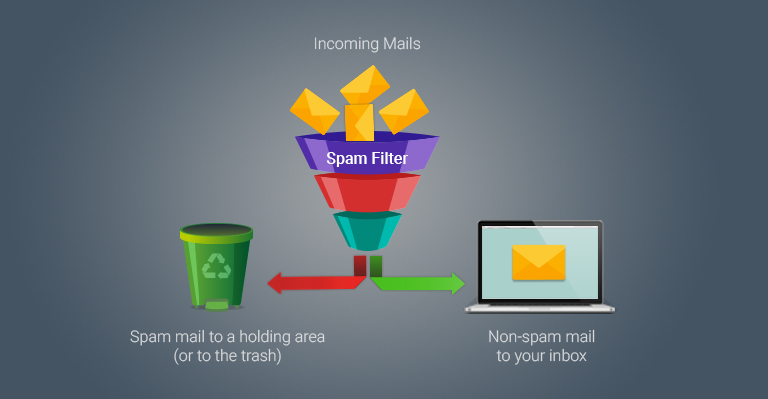
\includegraphics[width=0.7\linewidth]{pictures/anti-spam-filtering-techniques.png}
	\caption{One application of transfer learning: spam filtering}
	\label{fig:datree}
\end{figure}

Such examples motivate the domain adaptation problem and extend traditional learning paradigms. For the rest of this dissertation, we investigate the scenario where a model may be learned on one distribution but evaluated on another.

\section{Background}
For the applications considered previously, the goal is to find a model that remains robust under changes in the environment. In other words, if a model is learned from the source, we want to measure how well it performs on the target domain. Formally, we describe this as follows

\begin{theorem}[Transfer learning]
	Let $S$ be a source data distribution called the source domain and $T$ be a target data distribution called the target domain. Consider $X_S\times Y_S$ as the source input and output spaces and $X_T\times Y_T$ as target input and output spaces. Denote $S_X$ and $T_X$ to be the marginal distributions of $X_S$ and $X_T$ and by $t_S$ and $t_T$ the source and target learning tasks depending on $Y_S$ and $Y_T$ respectively. We seek to improve the performance of $f_{T}:X_T\to Y_T$ for $t_T$ using information gained from $S$ where $S\neq T$.
\end{theorem}

\subsection{Transfer learning scenarios}
 
Furthermore, we may have the following types:
\begin{itemize}
	\item Inductive transfer learning. $X_S=X_T$ but $t_S\neq t_T$.
	\item Transductive transfer learning. $X_S\neq X_T$ but $t_S=t_T$.
	\item Unsupervised transfer learning. $t_S\neq t_T$ and $X_S\neq X_T$.
\end{itemize}

The category we focus on is transductive transfer learning, which we call domain adaptation.

% TODO: \usepackage{graphicx} required
\begin{figure}
	\centering
	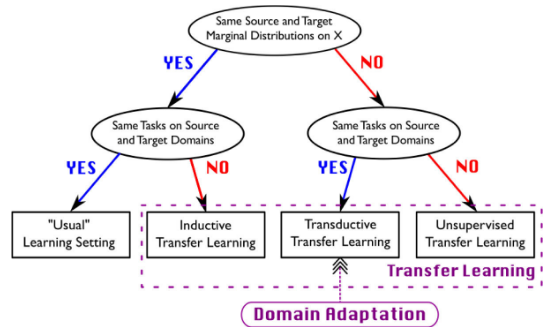
\includegraphics[width=0.7\linewidth]{pictures/DA_tree}
	\caption{Positioning of Domain Adaptation compared to other learning techniques (Redko)}
	\label{fig:datree}
\end{figure}

From a probabilistic point of view, we can categorize our problem via the causal link between labels and instances.

\begin{itemize}
	\item $X\to Y$ problems where the class label is causally determined by instance values. This comes up in image classification where the object description determines the label. The joint distribution can be decomposed into $P(X,Y)=P(X)P(Y|X)$.
	\item $Y\to X$ where this is the reverse. Class labels causally determine instance values. A good example here is in medicine where we observe disease symptoms but want to predict the disease (Redko). The joint decomposition here is $P(X,Y)=P(Y)P(X|Y)$.
\end{itemize}

It follows that we can categorize different types of transfer learning scenarios based on the probabilistic point of view. The following are some such scenarios:

\begin{itemize}
	\item Covariate-shift
	$P(X_S)\neq P(X_T)$ but $P(Y_T|X_T)= P(Y_S|X_S)$
	
	This is a case of the $X\to Y$ problem where $X_S\not\equiv X_T$ while $Y_S|X_S \equiv Y_T|X_T$. Here, the marginal distributions between the source and target are different while the predictive behavior stays the same. One example of this is the Office/Caltech dataset with domains:
	
	\begin{enumerate}
		\item Amazon images from online merchants
		\item Webcam low-quality images
		\item High-quality images by a DSLR
		\item Images from Caltech dataset for object recognition
	\end{enumerate}
	
	% TODO: \usepackage{graphicx} required
	\begin{figure}
		\centering
		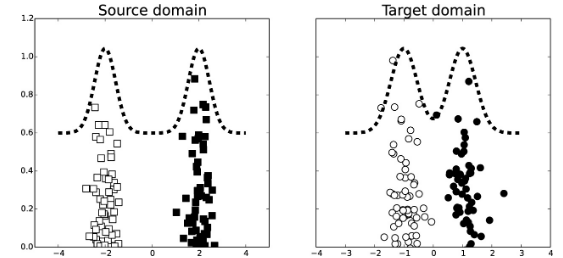
\includegraphics[width=0.7\linewidth]{pictures/covariate_shift}
		\caption[Covariate shift illustration]{Covariate shift}
		\label{fig:covariateshift}
	\end{figure}

	Solving the covariate shift problem involves a reweighting as seen by the following:
	
	\begin{align*}
	R^l_T(h) &= \E_{(x,y)\sim T} l(h(x),y) \\
	&= \E_{(x,y)\sim T} \frac{S(x,y)}{S(x,y)}l(h(x),y) \\
	&= \E_{(x,y)\in X\times Y} T(x,y)\frac{S(x,y)}{S(x,y)}l(h(x),y) \\
	&= \E_{(x,y)\sim S} \frac{T(x,y)}{S(x,y)}l(h(x),y) \\
	&= \E_{(x,y)\sim S} \frac{P(X_T)}{P(X_S)}l(h(x),y)
	\end{align*}
	
	where the last equality used the fact that $P(Y_T|X_T)=P(Y_S|X_S)$.
	
	
	\item Target-shift
	$P(X_T|Y_T)\neq P(X_S|Y_S)$
	
	These occur in $Y\to X$ problems. In this case, $Y_S\not\equiv Y_T$--the target distributions are different. Generally, this occurs when different sampling methods are used for the source and target datasets.
	
	\begin{figure}
		\centering
		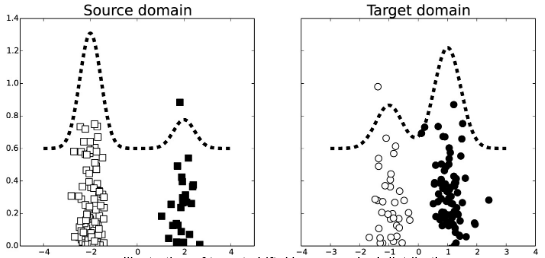
\includegraphics[width=0.7\linewidth]{pictures/target_shift}
		\caption[Target shift illustration]{Target shift}
		\label{fig:targetshift}
	\end{figure}
	
	\item Concept shift
	$P(X_T,Y_T)\neq P(X_S,Y_S)$ This occurs both in $X\to Y$ and $Y\to X$ problems when $P(Y_S|X_S)\neq P(Y_T|X_T)$ and $P(X_S|Y_S)\neq P(X_T|Y_T)$ respectively.
	\item Sample-selection bias
	
	Here, the source and target distributions differ because of a latent variable that excludes some sample observations conditional on their labeling or nature. For example, if we are classifying images of people, we may discard images that are unclear. This leads to a sample-selection bias since some devices may take more unclear pictures by default.
	
	\item Ideal joint error.
	We may claim the existence of a low-error hypothesis for both the source and target domain. Usually, this is characterized by
	\[
	\lambda_{\mathcal{H}}=\min_{h\in \mathcal{H}} R_S(h)+R_T(h)
	\]
	
\end{itemize}

As a side-note, there are three predominant algorithmic techniques used for domain adaptation. They are

\begin{itemize}
	\item Reweighting the source labeled examples to be more similar to the target examples. This is done in cases such as covariate shift.
	\item Iteratively "auto-labeling" target examples. Here, a model is learned from labeled examples and then automatically labels some target examples. We then learn a new model from the new labeled examples.
	\item Finding a common representation space. In this situation, we find a space where the source and target domains are close while maintaining a good performance on the source domain task.
\end{itemize}

\subsection{Divergence between domains}

In domain adaptation, we must define a dissimilarity measure between source and target domains. Unlike classical supervised learning, transfer learning involves a discrepancy between the two domains. There are many metrics such as Hellinger distance total-variation distance, Renyi divergence, or Wasserstein metric that exist to measure such a discrepancy, and the choice of metric can impact the behavior of the labeling function. 

Often, one wants to prove that a divergence measure can relate errors between source and target domains. Then this means we can establish error guarantees by minimizing the divergence between the source and target distributions.

Along with analyzing existing divergence measures, one may design a new divergence measure suitable for domain adaptation. This is done when a divergence measure is too difficult to compute empirically.  Additionally, chapter 3 of this dissertation investigates a new specific divergence measure.

In the subsequent paragraphs, we discuss seminal work in the topic. This is done to demonstrate better what we mean by relating errors between domains with respect to a divergence measure.

\subsection*{A First Theoretical Analysis}
From a theory perspective, the seminal work on this was done by Ben-David et al. In their work, they considered a binary loss function in a binary classification setting and proposed the $L^1$-distance.

First, let's provide some definitions.

\begin{definition}{Rademacher complexity}
	
	Given a sample $S=(z_1, z_2, \dots, z_m) \in Z^m$, and a class $F$ of real-valued functions defined on a domain space $Z$,
	\[
	\operatorname{Rad}_S(F) 
	= 
	\frac{1}{m}
	\operatorname{E} \left[
	\sup_{f \in F}
	\sum_{i=1}^m \sigma_i f(z_i) 
	\right]
	\]
\end{definition}

\begin{definition}{Shattering}
	
	A family $H$ shatters a set $S \subseteq \mathcal{X}$ if for every subset $T \subseteq S$ there exists a function $h \in H$ such that $h(s) = 1_{s \in T}$ for all $s \in S$, that is, $h(s) = 1$ if $s \in T$ and $h(s) = 0$ if $s \in S \setminus T$.
	
	Intuitively, we say that $H$ shatters some set $S \subseteq \mathcal{X}$ if we can realize any labelings on $S$ using functions from $H$.
	
\end{definition}

\begin{definition}{VC Dimension}
	 
	 The VC dimension of a set of hypothesis functions $H$ is the cardinality of the largest set which $H$ can shatter.
	
\end{definition}

\begin{definition}{$\mathcal{H}$-divergence}
	
	Denote $\mathcal{A}$ the set of measurable subsets under two probability distributions $\mathcal{D}$ and $\mathcal{D'}$. Then the $\mathcal{H}$-divergence is defined as
	\[
	d_{1}(\mathcal{D},\mathcal{D'}) = 2 \sup_{A\in \mathcal{A}} \left| P_D(A)-P_{D'}(A) \right| .
	\]
\end{definition}

This one compares how two classifiers disagree on both domains. Here, it finds the pair of classifiers with the largest disparity in disagreements between the source and target domains.

Using this notion of distance, Ben-David et al. derived the first generalization bounds.

\begin{theorem}{Ben-David et. al}
	
	Let $l$ represent the $0-1$ loss function and $f_S,\,f_T$ the source and target true labeling functions respectively.
	\[
	R_T^{l}(h) \leq R_S^{l}(h) + d_1(X_S,X_T) + \min \left\{ \E_{x\sim X_S} [\left\|f_S(x)-f_T(x)\right\|], \E_{x\sim X_T} [\left\|f_S(x)-f_T(x)\right\|] \right\}
	\]

\end{theorem}

This was the first theoretical generalization bound, but it had some flaws. In practice, one may want to obtain finite-sample estimates, but that isn't possible with $\mathcal{H}$-divergence. Also, the $\mathcal{H}$-divergence does not incorporate the hypothesis class considered. Both of these issues are resolved with the introduction of another type of divergence: the symmetric difference hypothesis divergence.

\begin{definition}{Symmetric difference hypothesis divergence}
	\[
	D_{\mathcal{H}\Delta \mathcal{H}}(S,T) = 
	2 \sup_{h,h'\in \mathcal{H}} \left| P_S[h(x)\neq h'(x)] - P_T[h(x)\neq h'(x)] \right| 
	\]
\end{definition}

\begin{theorem}
	Here, $\hat{S},\hat{T}$ are independent size-$m$ samples drawn from $S$ and $T$ respectively. For $\delta\in (0,1)$, the following holds with probability at least $1-\delta$:
	
	\[
	D_{\mathcal{H}\Delta \mathcal{H}}(S,T) \leq \hat{D}_{\mathcal{H}\Delta \mathcal{H}}(\hat{S},\hat{T}) + 
	4 \sqrt{\frac{2 VC(\mathcal{H}) \log(2m) + \log(2/\delta)}{m}}
	\]
\end{theorem}

The above tells us that, for a finite $VC$ dimension class $\mathcal{H}$, the empirical $\mathcal{H}\Delta \mathcal{H}$ divergence is a good estimate for its true variant.

Furthermore, one can compute the empirical divergence. Ben-David then obtained a bound for risk on the target domain that involved the empirical divergence.

\begin{theorem}
	Let $\lambda^* = \min_{h\in \mathcal{H}} R_S(h)+R_T(h)$ be the minimum joint risk.
	With probability at least $1-\delta$:
	
	\[
	R_T^l(h) \leq \hat{R}_S^l(h) + \frac{1}{2}D_{\mathcal{H}\Delta \mathcal{H}}(\hat{S},\hat{T}) + \lambda^{*} + 
	O \left( \sqrt{\frac{VC(\mathcal{H}) \log(m) + \log(2/\delta)}{m}}\right) 
	\]
\end{theorem}

One sees here that the bound relies on a notion of divergence between the two domains as stated earlier along with a divergence between the hypothesis and true labeling function.

Of note here is that the risk bound presented is only relevant if the optimal joint risk is controlled.

\subsection*{Critique of $\mathcal{H}\Delta\mathcal{H}$-divergence}

A flaw of the $\mathcal{H}\Delta\mathcal{H}$-divergence is that it relies on a specific loss function (0-1 loss). But one may want to work with more general loss function. This motivated other work by Mohri and Mansour to use Renyi and $\mathcal{Y}$-discrepancy distances.

\begin{definition}{Renyi divergence}
	\[
	D_{\alpha}(p,q) = \frac{1}{\alpha-1} \log_2 \int_{\mathcal{X}} p^{\alpha}(x)/q^{\alpha-1}(x) \, dx,
	\]
	where $\alpha$ denotes its order. When $\alpha=1$, the Renyi divergence is equivalent to the Kullback-Leibler divergence.
\end{definition}

\begin{definition}{$\mathcal{Y}$-Discrepancy}

	Let $f_P$ and $f_Q$ be the labeling functions on $P$ and $Q$. Then the $\mathcal{Y}$-discrepancy between domains $(P,f_P)$ and $(Q,f_Q)$ is
	\[
	\textrm{disc}_{\mathcal{Y}}(P,Q) = \sup_{h\in H} \abs{\mathcal{L}_Q(h,f_Q)-\mathcal{L}_P(h,f_P)}
	\]
\end{definition}

In our work, we study divergences inspired by optimal transport theory. This brings us to the next section, which introduces some of the foundational material on Wasserstein spaces.

\section{Brief Introduction to Optimal Transport}

\subsection*{Monge Problem}

In 1781, Gaspard Monge asked how one can transport a pile of sand into a pit when both have equal volumes.

Intuitively, the goal is to minimize the expected "cost" of moving the sand, and it turns out this has a mathematical formulation as follows:

Let $X$ be the space of sand, $Y$ be the space for the pit, and define a cost function $c:X\times Y\to \mathbb{R}$ that demonstrates the cost of moving a unit of sand $x\in X$ to a pit location $y\in Y$.

The choice of where to place a unit of sand can be represented as the function $T:X\to Y$, which has a total transport cost of
\[
\int_{X} c(x,T(x))\,d\mu(x).
\]

Here, the sand distribution and shape of the pit are represented by distributions $\mu$ and $\nu$ respectively.

Moreover, one cannot change the size of a sand particle, so the sand cannot be concentrated at a single point in the pit. In other words, the function $T$ must satisfy a mass-preservation requirement: the volume $\nu(B)$ of any region in the pit $B\subseteq Y$ must be the same as the volume of the sand moved into $B$.

Formally, we can write this as
\[ 
\mu(T^{-1}(B))=\nu(B) \text{ for all } B\subseteq Y
\] which we denote $T\#\mu=\nu$. We can also recognize this as $\nu$ is the push-forward measure of $\mu$ under $T$.

If $c$ and $T$ are measurable, and $\mu(T^{-1}(B))=\nu(B)$ for all measurable subsets $B$ of $Y$, then $T$ is a transport map. Normalizing $\mu$ and $\nu$ to be probability measures, the Monge problem finds the optimal transport map minimizing transport costs \cite{Panaretos2020}. 

\begin{definition}{Monge Problem}
	
	Let $T:X\to Y$ be a transport map with an associated total cost \[
	C(T) = \int_{X} c(x,T(x)) \,d\mu(x).
	\] where $\mu$ and $\nu$ are again the probability measures assigned to $X$ and $Y$.
	
	The Monge problem finds
	\[
	\inf_{T:T\#\mu=\nu} C(T).
	\]
\end{definition}

The Monge problem is very hard because the set of transport maps $\{T:T\#\mu = \nu\}$ is intractable to work with. Currently, if $\mu=\delta\{x_0\}$ is a Dirac measure and $\nu$ is not, then no transport maps exist.

But what if we can split the mass of sand particles? That is to say, we don't have the strict conditions as above. This brings us to the Kantorovich relaxation.

\subsection*{Kantorovich Relaxation}
For each point $x\in X$, a probability measure $\mu_x$ defines how the mass at $x$ is split. If $\mu_x = \delta\{y\}$ for $y\in Y$, then all the mass at $x$ is sent to $y$.

Represent $\pi$ to be the joint probability measure on $X\times Y$, where $\pi(A\times B)$ is the amount of sand moved from $A\subseteq X$ to $B\subseteq Y$. The total mass sent from $A$ is $\pi(A\times Y)$ and the total moved into $B$ is $\pi(X\times B)$. Such a measure $\pi$ is called a  transference plan when
\begin{align*}
\pi(A\times Y) = \mu(A),\quad A\subseteq X \\
\pi(X\times B) = \nu(B),\quad B\subseteq Y
\end{align*}

where $A$ and $B$ are Borel sets. The set of transference plans is denoted $\Pi(\mu,\nu)$.

\begin{definition}{Kantorovich Problem}
	
	Let $\pi\in \Pi(\mu,\nu)$ be a transference plan with an associated total cost \[
	C(\pi) = \int_{X\times Y} c(x,y) \,d\pi(x,y).
	\]
	
	The Kantorovich problem solves for the optimal plan given by
	\[
	\inf_{\pi\in \Pi(\mu,\nu)} C(\pi).
	\]
\end{definition}

\subsection*{Probabilistic Interpretations of Monge and Kantorovich Problems}
We can view the above optimization problems from a probabilistic perspective. The Monge solution minimizes  $\E_{X}[c(X,T(X))]$ over $T$ (measurable) whereas the Kantorovich solution minimizes $\displaystyle\E_{\pi\in \Pi(\mu,\nu)}[c(X,Y)].$ We call $\pi \in \Pi(\mu,\nu)$ a coupling between $X$ and $Y$.

\subsection*{A Divergence Measure Inspired by Optimal Transport}
If $X=Y$, then we can define a distance between measures $\mu$ and $\nu$ using a special cost function $c$. 

Let $c(x_1,x_2) = [d(x_1,x_2)]^p$, where $d(x_1,x_2)$ denotes the distance between $x_1$ and $x_2$ and $p$ is a real-valued constant

\begin{definition}{Wasserstein Distance of Order p}
	\[
	W_p(\mu,\nu) = \left( \inf_{\pi\in \Pi(\mu,\nu)} \int_{X\times X} d(x_1,x_2)^p \,d\pi(x_1,x_2)\right)^{1/p} = \left( \inf_{\pi\in \Pi(\mu,\nu)} \E_{\pi}[d(x_1,x_2)^p] \right)^{1/p} .
	\]
\end{definition}

With this being said, let's begin.
\chapter{Theoretical Analysis of Domain Adaptation with Sinkhorn Divergence}

In this chapter, we discuss some of our first results when using a entropic-based divergence. In the past, generalization bounds were provided with respect to the Wasserstein metric, but the empirical computation involved a regularization step, which was previously unaccounted for when deriving bounds. In this work, we provide a theoretical analysis of the generalization bound with respect to the entropic regularization in the unsupervised domain adaptation setting.

\section*{Why Use Optimal Transport in Domain Adaptation?}
Optimal transport is capable of taking into consideration the geometry of the data. In domain adaptation problems, this is helpful, especially since when dealing with a source and target distribution, a natural idea is to look for a nonlinear transformation between the two distributions. This makes optimal transport distances (i.e. Wasserstein) highly promising. Another concern is that the source and target distributions lack a shared support. It makes sense to use a distance that does not require a shared support and the Wasserstein is one such distance. This property distinguishes it from other divergences such as Maximum Mean Discrepancy or Kullback-Leibler, which usually require a common support.

\section{Notation and Preliminaries}

\begin{definition}{Reproducing Kernel Hilbert Space}
	
	Let $X$ be an arbitrary set and $H$ a Hilbert space of real-valued functions on $X$.  The evaluation functional over the Hilbert space of functions $H$ is a linear functional that evaluates each function at a point $x$,
	
	\[
	L_{x} : f \mapsto f(x)  \text{   } \forall f \in H.
	\]
	
	We say that $H$ is a reproducing kernel Hilbert space if, for all $x \in X$, $L_{x}$ is continuous at any $f\in H$ or, equivalently, if $L_x$ is a bounded operator on $H$, i.e. there exists some $M > 0$ such that
	
	\[
	|L_{x}(f)| := |f(x)| \le M \|f\|_H \quad \forall f \in H.
	\]

\end{definition}

\begin{definition}{Kullback-Leibler Divergence}
	If $P$ and $Q$ are probability measures on a set $\mathcal{X}$, and $P$ is absolutely continuous with respect to $Q$, then the Kullback-Liebler divergence from $Q$ to $P$ is
	\[
	D_{KL}(P \parallel Q)=\int_{\mathcal{X}} \log \left( \frac{dP}{dQ}\right) \, dP.
	\]
\end{definition}

\begin{definition}{Maximum mean discrepancy}
	
	MMD represents distances between distributions as distances between mean embeddings of features. If we have distributions $p$ and $q$ over a set $\mathcal{X}$, the MMD is defined by a feature map $\varphi: \mathcal{X}\to \mathcal{H}$ where $\mathcal{H}$ is a reproducing kernel Hilbert space.
	\[
	MMD(p,q) = \norm{ \E_{X\sim p}[\varphi(X)] - \E_{Y\sim q}[\varphi(Y)] }_{\mathcal{H}}
	\]
	
	We can alternatively characterize the MMD as follows:
	\begin{align*}
	MMD(p,q) &= \norm{ \E_{X\sim p}[\varphi(X)] - \E_{Y\sim q}[\varphi(Y)] }_{\mathcal{H}} \\
	&= \sup_{f\in \mathcal{H}:\norm{f}_{\mathcal{H}}\leq 1} \ang*{f,\E_{X\sim p}[\varphi(X)] - \E_{Y\sim q}[\varphi(Y)]}_{\mathcal{H}} \\
	&= \sup_{f\in \mathcal{H}:\norm{f}_{\mathcal{H}}\leq 1} \bkt*{\ang*{f,\E_{X\sim p}[\varphi(X)]}_{\mathcal{H}} - \ang*{f,\E_{Y\sim q}[\varphi(Y)]}_{\mathcal{H}} } \\
	&= \sup_{f\in \mathcal{H}:\norm{f}_{\mathcal{H}}\leq 1} \bkt*{ \E_{X\sim p}[f(X)] - \E_{Y\sim q}[f(Y)] }
	\end{align*}
\end{definition}

The alternative characterization holds because of the reproducing property: 
$\ang{f,\varphi(x)}_{\mathcal{H}}=f(x)$ for any
$f\in \mathcal{H}$. The second line holds since $\sup_{f:\norm{f}\leq 1} \ang{f,g}_{\mathcal{H}} = \norm{g}$ is attained when $f=g/\norm{g}$. The fourth relies on Bochner integrability, but assuming our kernel or distributional support is bounded, this is true. The last line is a byproduct of the reproducing property.

The following extension of Wasserstein to empirical measures will be used when contrasting empirical to theoretical distances.

\begin{definition}{Discrete Wasserstein} \cite{Redko2017}
	
	If we deal with empirical measures $\hat{\mu}_{S}=\frac{1}{N_{S}}\sum_{i=1}^{N_{S}}\delta_{x_{\mathrm{s}}^{i}}$ and $\hat{\mu}_{T}=\frac{1}{N_{T}}\sum_{i=1}^{N_{T}}\delta_{x_{T}^{i}}$ represented by the uniformly weighted sums of $N_{S}$ and $N_{T}$ Diracs with mass at locations $x_{S}^{i}$ and $x_{T}^{i}$ respectively, then the Kantorovich problem is defined in terms of the inner product between the coupling matrix $\gamma$ and the cost matrix $C$:
	
	$$
	W_{1}(\hat{\mu}_{S},\hat{\mu}_{T})=\min_{\gamma\in\Pi(\hat{\mu}_s,\hat{\mu}_{T})} \langle C,\ \gamma\rangle_{F}
	$$
	
	where $\langle \, , \, \rangle_F$ denotes the Frobenius inner product, $\Pi(\hat{\mu}_s,\hat{\mu}_{T})=\{\gamma\in \mathbb{R}_{+}^{N_{\mathrm{S}}\times N_{T}}|\gamma 1=\hat{\mu}_{S}, \gamma^{T}1= \hat{\mu}_{T}\}$ is a set of doubly stochastic matrices and $C$ is a dissimilarity matrix, i.e., $C_{ij}= c(x_{S}^{i},\ x_{T}^{j})$, defining the energy needed to move a probability mass from $x_{S}^{i}$ to $x_{T}^{j}$.
	
\end{definition}

\begin{definition}[Expected Loss]
	Let $l$ be a convex loss-function. Given a distribution $\mu_D$, a hypothesis $h\in H$ and a labeling function $f_D$ (which may be a hypothesis), the expected loss is defined as
	
	\[
	\epsilon_D(h,f_D) = \E_{X\sim \mu_D}[l(h(x),f_D(x))].
	\]
\end{definition}

\medskip

Our source and target spaces are denoted by $S$ and $T$ respectively. $S$ has a distribution $\mu_S$ and $T$ has as its underlying distribution, $\mu_T$. Our loss function is denoted by $\ell: \mathbb{R}\times \mathcal{Y}\to \mathbb{R}^{+}$.

We also use a $\Gamma$ operator to represent expectation, i.e. $\Gamma f = E_{\pi}[f(X)]$ where $X\sim \pi$.

\medskip


The following interpretation of expected loss using RKHS properties was used to derive earlier bounds.

\begin{definition}[RKHS interpretation]
	Assume $l \in \mathcal{H}_{k^q}$ where $\mathcal{H}_{k^q}$ is an RKHS with kernel $k^q: \Omega\times \Omega\to \mathbb{R}$ induced by $\phi: \Omega\to \mathcal{H}_{k^q}$ and $k^q(x,y) = \ang*{\phi(x),\phi(y)}_{\mathcal{H}_{k^q}}$.
	
	With this definition, it is immediate that,
	$$ \epsilon_S(h,f_S) = \E_{x\sim \mu_S}\bkt*{l(h(x),f_S(x))} = \E_{x\sim \mu_S}\bkt*{\ang*{\phi(x),l}_{\mathcal{H}_{k^q}}} $$
	
	and
	
	$$ \epsilon_T(h,f_T) = \E_{y\sim \mu_T}\bkt*{l(h(y),f_T(y))} = \E_{y\sim \mu_T}\bkt*{\ang*{\phi(y),l}_{\mathcal{H}_{k^q}}} .$$
\end{definition}

\section*{Prior Work}

First, we introduce some past results pertaining to risk bounds with respect to the Wasserstein distance. As we will see, the choice of the cost function is key in deriving theoretical bounds.

\subsection*{First Theoretical Bounds \cite{Redko2017}}
The key assumption here is that of the cost function. Another assumption here is that the true labeling function $f$ lies within a unit ball of an RKHS, i.e. \[\mathcal{F} = \{f\in \mathcal{H}_k: \, \norm{f}_{\mathcal{H}_k}\leq 1\},\] where $\mathcal{H}_k$ is an RKHS with kernel $k$.

In this scenario, we have the following specifications:
\begin{itemize}
	\item Let $\mu_S, \mu_T\in \mathcal{P}(X)$ be two probability measures on $\mathbb{R}^d$.
	\item \[c(x,x') = \norm*{\phi(x)-\phi(x')}_{\mathcal{H}_{k_l}}.\] 
	\begin{itemize}
		\item $\mathcal{H}_{k_l}$ is an RKHS.
		\item $k_l: \Omega\times \Omega\to \mathbb{R}$ is a kernel function such that \[k_l(x,x')=\ang*{\phi(x),\phi(x')}_{\mathcal{H}_{k_l}}\]
	\end{itemize}
	\item \[l(h(x),f(x)) = \abs*{h(x)-f(x)}^q,\, q>0\] and thus the loss function is convex, bounded, symmetric, and satisfies triangle inequality
	\item If $\Omega$ is separable and $k_l(x,x')\in [0,K]$ for some $K\in \mathbb{R}$, then for all $x,x'\in \Omega$,
	\[
	\E_D[\sqrt{k_l(x,x')}]<\infty
	\] for $D=S$ or $T$.
\end{itemize}

Before we continue, let us briefly discuss the use of the aforementioned cost function. One sees that

\begin{align*}
c(x,x')&=\norm{\phi(x)-\phi(x')}_{\mathcal{H}} \\
&= \sqrt{\ang{\phi(x)-\phi(x'),\phi(x)-\phi(x')}_{\mathcal{H}}} \\
&= \sqrt{k(x,x)-2k(x,x')+k(x',x')}.
\end{align*}

One can show there is a one-to-one relationship between the choice of a positive-definite kernel $k$ and the cost function $c$.

Secondly, $l_{h,f}:x\to l(h(x),f(x))$ belongs to an RKHS. $(h,f)\in \mathcal{F}^2$ and $l$ is a nonlinear mapping of $\mathcal{H}_k$.

\medskip

\begin{lemma}
	If the above assumptions hold, then, for all $h,f\in \mathcal{H}_{k_l}$, 
	\[ \epsilon_T(h,f)\leq \epsilon_S(h,f) + W_1(\mu_S,\mu_T). \]
\end{lemma}

With the use of a concentration inequality on Wasserstein distances \cite{Bolley2007}, empirical risk bounds are obtained.

\begin{theorem}
	Let $\mu$ be a probability measure on $\mathbb{R}^d$ such that
	\[
	\int_{\mathbb{R}^d} e^{\alpha \norm{x}^2}\,d\mu < \infty, \, \exists \alpha > 0
	\]
	and let $\hat{\mu}=\frac{1}{N}\sum_{i=1}^N \delta_{X_i}$ be the empirical measure on $\{x_i\}$.
	
	Then for all $d'>d$ and all $\xi < \sqrt{2}$, there exists $N_0(d')$ and $\alpha > 0$ with
	\[
	\int e^{\alpha c(x,x')}\,d\mu(x) < \infty
	\]
	for a fixed $x'$ such that for all $\epsilon > 0$ and all $N\geq N_0 \max \{\epsilon^{-(d'+2),1}\}$,
	
	\[
	\Pr[W_1(\mu,\hat{\mu})>\epsilon] \leq e^{-\frac{\xi}{2} N\epsilon^2}
	\]
\end{theorem}

\subsection*{Joint Distribution Domain Adaptation (JDOT)}
This is the approach taken in \cite{Courty2017} and also the problem we study in the rest of this chapter with regularization. In this setting, one works with unsupervised domain adaptation between joint distributions. The inspiration behind this method is that the assumption that  conditional distributions are preserved, i.e. $P_S(Y|T(X))\approx P_T(Y|T(X))$, may not necessarily hold.
\begin{itemize}
	\item Now the cost function used is \[\alpha d(x_s,x_t) + L(y_s,y_t).\]
	\item The unsupervised domain adaptation problem is studied here, so the target labels represented by $y_t$ are not known. Thus, one cannot find an optimal coupling.
	\item It does not matter that an optimal coupling is not found since the goal here is to estimate a mapping on the target data.
\end{itemize}
%%EDIT THIS MORE
%fix citation

%end
\section*{Uniform empirical risk bounds on RKHS}
Using properties of the Rademacher complexities of functions in an RKHS, we can avoid bounding empirical risks w.r.t Wasserstein distance.

$$ \sup_{f\in F} \abs{\E f(X) - \frac{1}{n}\sum_{i=1}^n f(X_i)} = \norm{P-P_n}_F. $$

$$ \E \norm{P-P_n}_{F}\leq 2\norm{R_n}_F $$

Let $F = \left\{f\in \mathcal{H} | \norm{f}_{H}\leq B\right\}$

$$ \E \bkt*{\norm{R_n}_{F} | X_1,\ldots,X_n} \leq \frac{B}{\sqrt{n}} \sqrt{\frac{tr(K)}{n}}. $$

\begin{proof}
	\begin{align*}
	\norm{R_n}_F &= \sup_{f\in F} \abs*{ \frac{1}{n} \sum_{i=1}^n \epsilon_i f(X_i)} \\
	&= \sup_{f\in F} \abs{\frac{1}{n} \sum_{i=1}^n \epsilon_i \ang*{k(X_i,\cdot),f}} \\
	&= \sup_{f\in \mathcal{H}:\norm{f}_{\mathcal{H}}\leq B} \abs*{\ang*{\frac{1}{n}\sum_{i=1}^n \epsilon_i k(X_i,\cdot),f}} \\
	&= B\sqrt{\frac{1}{n^2} \sum_{i,j} \epsilon_i \epsilon_j k(X_i,X_j)}
	\end{align*}
	
	By Jensen's
	
	\begin{align*}
	\E \bkt*{ \norm{R_n}_F | X_{1}^{n}} &\leq B\sqrt{\E \bkt*{\frac{1}{n^2} \sum_{i,j} \epsilon_i \epsilon_j k(X_i,X_j)|X_{1}^{n}}} \\
	&= B \sqrt{\frac{1}{n^2} \sum_i k(X_i,X_i)} \\
	&= \frac{B}{\sqrt{n}} \sqrt{\frac{tr(K)}{n}}
	\end{align*}
\end{proof}

%\begin{align*}
%\norm{R_n}_F &= \sup_{f\in F} \abs*{ \frac{1}{n} \sum_{i=1}^n \epsilon_i f(X_i) \\
%	&= \sup_{f\in F} \abs{\frac{1}{n} \sum_{i=1}^n \epsilon_i \ang*{k(X_i,\cdot),f}} \\
%	&= \sup_{f\in \mathcal{H}:\norm{f}_{\mathcal{H}}\leq B} \abs*{\ang*{\frac{1}{n}\sum_{i=1}^n \epsilon_i k(X_i,\cdot),f}}
%\end{align*}

Taking expectations of both sides,
$$ \E \bkt*{\norm{R_n}_{F}}\leq \frac{B}{n}\E \bkt*{\sqrt{tr(K)}} $$

and if our kernel $k$ is bounded above by $M$, then
$$ \E \bkt*{ \norm{R_n}_F } \leq \frac{B}{n} \sqrt{nM} = B\sqrt{M/n}. $$

\section{Generalization Bounds}
\label{generalization-bounds}

Our claim is that we can get guarantees when doing a dual minimization of the Wasserstein distance with the specified cost function $\alpha d(x_s,x_t) + l(y_s,f(x_t))$ from $S$ to $T_{f}$. 
\[
(\hat{\Gamma},\hat{f})=\arg\min_{\Gamma,f}\Gamma\left[\alpha d(x_{s},x_{t})+l(y_{s},f(x_{t}))\right]
\]
over all couplings that preserve the marginals on $S$ ($x_{s},y_{s})$ and $T_{X}$ $(x_{t})$. Let $\hat{\Gamma}$ be the optimal joint distribution over $(x_{s},y_{s},x_{t})$ above. Now define $\hat{\hat{\Gamma}}$ on $(x_{s},y_{s},x_{t},y_{t})$ to be a coupling with the same marginal over $(x_{s},y_{s},x_{t})$ as $\hat{\Gamma}$ and the correct marginals on $T$ ($x_t,y_t$). Let $\Gamma^{*}$ be an arbitrary coupling on the same variables which preserves the marginal distributions on $S$ ($x_{s},y_{s}$)and $T$ (i.e., $x_{t},y_t$). For now, let's assume we're dealing with absolutely continuous distributions here so we don't have existence issues. Fix $f^*\in F$.

The main results in this paper are bounds on the expected loss with respect to Sinkhorn and Wasserstein divergences.

\subsection{Error bounds with respect to Wasserstein distance}
\begin{theorem}
	\[
	err_{T}(\hat{f}) \leq err_{T}(f^{*})+W(S,T)+\hat{\hat{\Gamma}}\left(-\alpha d(x_{s},x_{t})+l(y_{s},y_{t})\right)
	\] where $\hat{\hat\Gamma}$ is the expectation operator with respect to a coupling with matching marginals on $T$ and the same marginal on $(x_s,y_s,x_t)$ as $\hat{\Gamma}$.
\end{theorem}

\begin{proof}
	\begin{align*}
	err_{T}(\hat{f}) &= \hat{\hat{\Gamma}} l (y_t,\hat f(x_t)) \\
	& \leq \Gamma^{*}\left[\alpha
	d(x_{s},x_{t})+l(y_{t},f^{*}(x_{t}))+l(y_{t},y_{s})\right]
	- \hat{\hat{\Gamma}}\left[\alpha d(x_{s},x_{t})-l(y_{s},y_{t})\right] \\
	& = err_{T}(f^{*})+\alpha\left(\Gamma^{*}d(x_{s},x_{t})
	-\hat{\hat{\Gamma}}d(x_{s},x_{t})\right)
	+\Gamma^{*}l(y_{s},y_{t})+\hat{\hat{\Gamma}}l(y_{s},y_{t}).
	\end{align*}
	
	There, by choosing $\Gamma^*$ as the optimal coupling between $S$ and $T$, that is,
	\[
	W(S,T) = \Gamma^*\left(\alpha d(x_{s},x_{t}) +
	l(y_{s},y_{t})\right),
	\]
	then we get the upper bound
	\begin{align*}
	err_{T}(\hat{f})
	& \leq err_{T}(f^{*})+W(S,T)+\hat{\hat{\Gamma}}\left(-\alpha
	d(x_{s},x_{t})+l(y_{s},y_{t})\right).
	\end{align*}
\end{proof}

\subsection{Entropic Regularization}

One means of addressing the intractability of OT is by using an entropic regularization.

\begin{definition}[Entropic Regularization of Wasserstein]
	$$W_{\epsilon}(\alpha,\beta) = \min_{\pi \in \Pi(\alpha,\beta)} \int_{\mathcal{X}\times \mathcal{Y}} c(x,y)d\pi(x,y) + \epsilon H(\pi | \alpha \otimes \beta)$$
	where $$H(\pi | \alpha \otimes \beta) = \int_{\mathcal{X}\times \mathcal{Y}} \log \paren{\frac{d\pi(x,y)}{d\alpha(x)d\beta(y)}}d\pi(x,y).$$
\end{definition}

If we use the relative entropy as a regularizer, then we can formulate the dual of regularized OT as the maximization of an expectation problem \cite{Genevay2018}.

\begin{align*}
W_{\epsilon}(\alpha,\beta) &=\max_{u\in C(\mathcal{X}),v\in C(\mathcal{Y})}\int_{\mathcal{X}} u(x)\mathrm{d}\alpha(x)+\int_{y}v(y)\mathrm{d}\beta(y) \\
&-\varepsilon \int_{\mathcal{X}\times \mathcal{Y}} e^{\frac{u(x)+v(y)-c(x,y)}{\epsilon}}\mathrm{d}\alpha(x)\mathrm{d}\beta(y) + \varepsilon\\
&= \max_{u\in C(\mathcal{X}),v\in C(\mathcal{Y})} \mathrm{E}_{\alpha \otimes \beta} [f_{\epsilon}^{XY}(u,\ v)]+\epsilon
\end{align*}


where $f_{\epsilon}^{xy}(u,\ v)=u(x)+v(y)- \epsilon e^{\frac{u(x)+v(y)[minus]\mathrm{c}(x,y)}{\epsilon}}.$

Since $W_{\epsilon}(\alpha,\alpha)\neq 0$, we can normalize this by defining the Sinkhorn divergence as in the definition below.
\begin{definition}[Sinkhorn Divergence]
\[
\bar{W}_{\epsilon}(\alpha,\beta)=W_{\epsilon}(\alpha,\beta)-\frac{1}{2}(W_{\epsilon}(\alpha,\alpha)+W_{\epsilon}(\beta,\beta))
\] 
\end{definition}

\subsection{Sample Dependent Sinkhorn Bounds}

The keys for achieving generalization bounds in this section are the following two lemmas \cite{Genevay2018}: 
\begin{lemma}
	\label{divergence_sinkhorn_from_wasserstein}
	Let $\alpha$ and $\beta$ be probability measures on $\mathcal{X}$ and $\mathcal{Y}$ subsets of $\mathbb{R}^d$ such that $\abs{X}=\abs{Y}\leq D$ and assume that $c$ is L-Lipschitz w.r.t $x$ and $y$. Then
	$$W_{\epsilon}(\alpha,\beta)-W(\alpha,\beta) \leq 2\epsilon d \log \paren*{\frac{\epsilon^2 L D}{\sqrt{d}\epsilon}}$$ where $\mathcal{X}$ and $\mathcal{Y}$ are subsets of $\mathbb{R}^d$ with diameters at most $D$ and $c$ is $L$-lipschitz w.r.t $x$ and $y$.
\end{lemma}

and

\begin{lemma}
	Let $\hat{\alpha_n}$ and $\hat{\beta_n}$ be empirical measures for $\alpha$ and $\beta$ with size $n$ for each.
	
	\[
	\abs{W_{\epsilon}(\hat{\alpha_n},\hat{\beta_n})-W_{\epsilon}(\alpha,\beta)} \leq 6B \frac{\lambda K}{\sqrt{n}} + C\sqrt{\frac{2 \log\frac{1}{\delta}}{n}}
	\] with probability at least $1-\delta$.
\end{lemma}

\subsection*{New Generalization Bound}

\subsection*{Applying regularization to our minimization problem}

%Let's try to minimize
%\[
%(\hat{\Gamma},\hat{f})=\arg\min_{\Gamma,f}\Gamma\left[\alpha d(x_{s},x_{t})+l(y_{s},f(x_{t}))\right]+H(\pi(\Gamma)|S\otimes T_X)
%\]
%
%and see how the expression compares to \[
%\Gamma_n \left[\alpha d(x_{s},x_{t})+l(y_{s},f(x_{t}))\right]+H(\pi(\Gamma_n)|S\otimes T_X)
%\]
%
%To clarify here, $\Gamma$ is the operator representing expectation w.r.t the joint distribution, $\pi(\Gamma)$.
%
%\begin{align*}
%\hat{\hat{\Gamma}}\left[\alpha
%d(x_{s},x_{t})+l(y_{t},\hat{f}(x_{t}))-l(y_{s},y_{t})\right] + H(\pi(\hat{\hat{\Gamma}})|S\otimes T_X) & \leq
%\hat{\hat{\Gamma}}\left[\alpha
%d(x_{s},x_{t})+l(y_{s},\hat{f}(x_{t}))\right] + H(\pi(\hat{\hat{\Gamma}})|S\otimes T_X) \\
%& =\hat{\Gamma}\left[\alpha d(x_{s},x_{t})+l(y_{s},\hat{f}(x_{t}))\right] + H(\pi(\hat{\Gamma})|S\otimes T_X)\\
%&\leq \hat{\Gamma}_n (\alpha d(x_s,x_t) + l(y_s,\hat{f}(x_t))) + \epsilon + ? \\
%& \leq \Gamma_n^{*} (\alpha d(x_s,x_t) + l(y_s,f^{*}(x_t))) + \epsilon + \epsilon + ?\\
%&\leq\Gamma^{*}\left[\alpha d(x_{s},x_{t})+l(y_{s},f^{*}(x_{t}))\right] + 2\epsilon + ?\\
%& \leq\Gamma^{*}\left[\alpha d(x_{s},x_{t})
%+l(y_{t},f^{*}(x_{t}))+l(y_{t},y_{s})\right] + 2\epsilon + ?
%\end{align*}

Letting $c_f(x_s,y_s,x_t) = \alpha d(x_s,x_t) + l(y_s,f(x_t))$, we'll apply the technique from Geneway's paper "Sample Complexity of Sinkhorn Distances" to give sample bounds on the Sinkhorn distance.

The difference here is we'll also show that our $f_{\epsilon}$ is lipschitz in $f$, which comes up in $c_f$ defined earlier.

$$W_{\epsilon}(S,T_X) = \max_{u\in c(S),v\in c(T_X)} \E_{S\otimes T_X} [f_{\epsilon}^{S,T_X}(u,v)]+\epsilon$$

$$f_{\epsilon}^{S,T_X}(u,v) = u(x_s,y_s)+v(x_t)-\epsilon \exp \paren*{\frac{u(x_s,y_s)+v(x_t)-c(x_s,y_s,x_t)}{\epsilon}}$$

$$c_f(x_s,y_s,x_t) = \alpha d(x_s,x_t)+l(y_s,f(x_t))$$
$$u(x_s,y_s)\leq L\norm{(x_s,y_s)}$$
$$v(x_t) \leq \max_{x_s,y_s} u(x_s,y_s)-c_f(x_s,y_s,x_t)$$

Things to note here:
I need to check if it matters that $S$ and $T_X$ have different dimensions because in the paper, the two had equal dimension. Now, I'm using $S$ to replace $\mathcal{X}$ and $T_X$ for $\mathcal{Y}$.

We also know that on the subset where $u$ and $v$ are optimal, $u\oplus v\leq 2L\norm{S}+\norm{c}_{\infty}$. Call this subset $\mathcal{A}$.

And let $Q=\exp \paren*{\frac{u(x_s,y_s)+v(x_t)-c(x_s,y_s,x_t)}{\epsilon}}$ so $\abs{Q}\leq \exp\paren{2\frac{L\abs{S}+\norm{c}_{\infty}}{\epsilon}}.$

$$\frac{\partial f_{\epsilon}}{\partial f} = -\epsilon \frac{\partial Q}{\partial f} = -\epsilon \cdot Q \cdot (1/\epsilon) \cdot \frac{\partial c}{\partial f} = -Q \frac{\partial c(f)}{\partial f} = -Q \frac{\partial l(f)}{\partial f}$$

Thus $$\abs{\frac{\partial f_{\epsilon}}{\partial f}}\leq \abs{Q}M,$$ as long as $\abs{l'(f)} \leq M.$

The above shows that if our loss function $l$ is Lipschitz w.r.t. $f$, then so is $f_{\epsilon}$ and we can then apply \ref{divergence_sinkhorn_from_wasserstein}, as long as $f$ is in an RKHS. To be more precise, $\norm{\nabla f^{\epsilon}(u,v)}\leq \max(1+M,\abs{Q}M)$.

Also recall $\norm{u}_{H^s}=O(1+\frac{1}{\epsilon^{s-1}})$ and $\norm{v}_{H^s}=O(1+\frac{1}{\epsilon^{s-1}})$ and we have, by using

$$ \E \bkt{\sup_{g\in G} \E l(g,X) - \frac{1}{n} \sum l(g,X_i)} \leq 2B\E R(G(X_1^n)) $$,

$$ \E \abs{W_{\epsilon}(\alpha,\beta) - W_{\epsilon}(\hat{\alpha_n},\hat{\beta_n})} \leq 3 \frac{2B\lambda}{n} \E \sqrt{\sum_{i=1}^n k(X_i,X_i)} $$

where $B\leq \max(1+M,\abs{Q}M)$, $\lambda$ is bounded since the norms of the potentials are bounded by $O(\max(1,\frac{1}{\epsilon^{d/2}}))$ and $f$ has bounded norm as well (still need to figure out an exact upper bound here).

After justifying the above two lemmas, we can then provide bounds w.r.t $W_{\epsilon}$ because

$$err_{T}(\hat{f}) + 4\epsilon d + 2\epsilon d \log(\frac{LD}{\sqrt{d}\epsilon}) \leq err_{T}(f^{*})+W_{\epsilon}(S,T)+\hat{\hat{\Gamma}}\left(-\alpha
d(x_{s},x_{t})+l(y_{s},y_{t})\right)$$

%\section*{Interpolation Between OT and MMD}
%Depending on the regularization strength $\epsilon$, we can %interpolate between OT and MMD using the Sinkhorn.

\chapter{An Alternative Means of Regularization for Domain Adaptation Problems}

\section*{Introduction}
Previously, we explored applications of entropic regularization for the Wasserstein distance (Sinkhorn) in domain adaptation. In particular, we derived a new generalization bound for target error with respect to the Sinkhorn divergence. However, for domain adaptation, entropic regularization may not be the ideal route to take.
 
When we prescribe a divergence measure for domain adaptation, the scenario we seek to penalize against is when the source $S$ and target $T$ distributions are not identical. However, with the entropic regularization, one is penalizing against $S$ and $T$ being independent. In this chapter, we propose an alternative regularization that may be more suitable for domain adaptation problems.

If $S$ and $T$ are identical in distribution, which is the ideal setting in machine learning, then there exists an identity mapping between the two. Thus, it makes sense to use a regularization that penalizes the deviation between our transport map and the identity map.

\newpage

\section*{Existence and Uniqueness of an Optimal Transport Map}
Our approach relies on Brenier's theorem, which concerns the existence and uniqueness of optimal maps.

\begin{theorem}{Brenier's Theorem}
	
	Let $\mu$ and $\nu$ be absolutely continuous probability measures on $\mathbb{R}^d$ with respect to the Lebesgue measure and $\nu$ has bounded support. There exists a convex function $\phi: \mathbb{R}^d\to \mathbb{R}$ such that its gradient, $\nabla \phi$, is the optimal transport map from $\mu$ to $\nu$.  
	
\end{theorem}

We call $\phi$ a Kantorovich potential.

\begin{corollary}{Existence of Solution to Monge Problem}
	
Under the above assumptions, $\nabla \phi$ uniquely solves the Monge problem.

\[
\int_X \abs{x-\nabla\phi(x)}^2\,d\mu(x) = \int_{T_{\#}\mu=\nu}\abs{x-T(x)}^2\,d\mu(x)
\]
	
\end{corollary}

\section*{Convex Analysis Prerequisites}

Before we continue, we introduce some concepts from convex analysis that will be needed going forward.

\begin{definition}
	Let $f:\,X\to \mathbb{R}\cup +\infty$ be a lower semicontinuous function. The Fenchel-Legendre transform $f^{*}: X^{*}\to \mathbb{R}\cup +\infty$ is defined by
	$$
	f^{*}(x^{*}) = \sup_{x\in X} [\ang*{x^{*},x}-f(x)]
	$$
	
	This $f^{*}$ is always convex.
\end{definition}

\begin{definition}
	The subdifferential of a lower semi-continuous convex function $\phi$ at $x\in \textrm{dom} \phi$ is defined by
	
	$$
	\partial \phi(x) = \{ x^{*}\in X^{*}: \phi(y)-\phi(x)\geq \ang*{x^{*},y-x} \}
	$$
\end{definition}

\begin{corollary}
	Let $f:\,X\to \mathbb{R}\cup \{+\infty\}$ be a convex function. Then for any $x\in \textrm{int dom }f$,
	
	$$ \partial f(x)\neq \emptyset.$$
\end{corollary}

\begin{theorem}[Fenchel-Young inequality]
	$$f(x)+f^{*}(x^{*})\geq \ang*{x^{*},x}$$
\end{theorem}

\begin{corollary}[Fenchel-Young equality]
	$$f(x)+f^{*}(x^{*})= \ang*{x^{*},x}$$ iff
	$$x^{*}\in \partial f(x).$$
\end{corollary}

\begin{theorem}
	Let $v(y) = \inf_x [f(x)+g(x+y)].$ The Fenchel primal problem is
	$$p = v(0) = \inf_x [f(x)+g(x)].$$
	
	The dual problem is
	$$d = v^{**}(0)=\sup_{y^{*}} [-f^{*}(y^{*})-g^{*}(-y^{*})].$$
\end{theorem}

\begin{proof}
	Calculate $v^{*}(-y^{*}) = \sup_{x,y}[\ang*{-y^{*},y}-f(x)-g(x+y)].$
	
	Let $u = x+y$, so we have
	\begin{align*}
	v^{*}(-y^{*}) &= \sup_{x,u} \ang*{-y^{*},u-x} - f(x) - g(u) \\
	&= \sup_x [\ang*{y^{*},x}-f(x)]+\sup_u [\ang*{-y^{*},u}-g(u)] \\
	&= f^{*}(y^{*}) + g^{*}(-y^{*}).
	\end{align*}
	
	Thus,
	$$d = v^{**}(0) = \sup_{-y^{*}}[0 - v^{*}(-y^{*})] = \sup_{-y^{*}}[-f^{*}(y^{*})-g^{*}(-y^{*})].$$
	
	Weak duality $p\geq d$ follows immediately. Strong duality $p=d$ requires $\partial v(0)\neq \emptyset$, i.e.
	$$0\in \textrm{int dom }v = \textrm{int}[\textrm{dom } g-\textrm{dom} f].$$
\end{proof}

\begin{proof}[Strong duality criterion]
	Here we prove $0\in \textrm{int dom }v = \textrm{int}[\textrm{dom } g-\textrm{dom} f]$ implies $\partial v(0)\neq \emptyset$. Let $-y^{*}\in \partial v(0)$ we have
	$$
	f(x)+g(x+y)\geq v(y)\geq p-\ang*{y^{*},y}
	$$
	Letting $u=x+y$, we have
	$$p\leq f(x)-\ang*{y^{*},x}+g(u)+\ang*{y^{*},u}
	$$ and taking infimum with respect to $x,u$, we have
	$$
	p\leq -f^{*}(y^{*})-g^{*}(-y^{*})\leq d\leq p.
	$$
	This concludes the proof.
\end{proof}

\section*{Derivation of Primal Formulation}

The goal is to find the primal formulation for the following optimization problem: 
$$ \inf_{u,v} \left[ \int u \, ds + \int v \, dt + \lambda (\norm{u}_H^2 + \norm{v}_H^2)\right],\, \frac{1}{2}\norm{x}^2 + \frac{1}{2}\norm{y}^2 - u(x) - v(y)\leq c(x,y). $$ The arguments that follow are similar to those used to prove Kantorovich duality.

Let $$\phi_c = \{ (u,v) \in C(X)\times C(Y): \frac{1}{2}\norm{x}^2 + \frac{1}{2}\norm{y}^2 - u(x) - v(y)\leq c(x,y)\}$$.
%$E^{*} = M(X\times Y)$ is the set of regular Radon measures with total variation norm.

In the next few lines, $z \in E = C(X\times Y)$ is the set of continuous functions on $X\times Y$ with sup. norm and $\pi\in E^{*} = M(X\times Y)$ is the set of regular Radon measures with total variation norm.

$$f(z) = \begin{cases}
\lambda( \left\|u\right\|_H^2 + \left\|v\right\|_H^2) + \int u\,ds + \int v\,dt, \, z(x,y)=u(x)+v(y) \\
+\infty, \, \textrm{ otherwise.}
\end{cases}$$

$$g(z) = \begin{cases}
0, \, \frac{1}{2}\norm{x}^2 + \frac{1}{2}\norm{y}^2 - z(x,y)\leq c(x,y) \\
+\infty, \, \textrm{ otherwise.}
\end{cases}$$

$$f(z)+g(z) = \begin{cases}
\int_X u\,ds + \int_Y v\,dt + \lambda(\left\|u\right\|_H^2 + \left\|v\right\|_H^2), \, \frac{1}{2}\norm{x}^2 + \frac{1}{2}\norm{y}^2 - u(x) - v(y)\leq c(x,y) \\
\infty, \textrm{ otherwise.}
\end{cases}$$

$$\inf_{z\in E} [f(z)+g(z)] = \inf_{(u,v)\in \Phi_c} \left\{ \int_X u\,ds + \int_Y v\,dt + \lambda(\left\|u\right\|_H^2 + \left\|v\right\|_H^2) \right\}$$

\begin{align*}
g^{*}(-\pi) &= \sup_{z\in E} \left[ -\int_{X\times Y} z\,d\pi - g(z)\right] \\
&= \sup_{z\in E} \left[ - \int_{X\times Y} z\,d\pi :\, \frac{1}{2}\norm{x}^2 + \frac{1}{2}\norm{y}^2 - c(x,y)\leq z(x,y) \right] \\
&= \begin{cases}
\int_{X\times Y} \left[c(x,y) - \frac{1}{2}\norm{x}^2 - \frac{1}{2}\norm{y}^2\right] \,d\pi,\, \pi\in M_{+}(X\times Y) \\
+\infty, \, \textrm{otherwise}
\end{cases}
\end{align*}

\begin{align*}
f^{*}(\pi) &= \sup_{z\in E} \left[ \int_{X\times Y} z\,d\pi - f(z)\right] \\
&= \sup_{z\in E} \left[ \int_{X\times Y} z(x,y)\,d\pi(x,y) - \int_X u\,ds - \int_Y v\,dt - \lambda(\left\|u\right\|_H^2 + \left\|v\right\|_H^2) :\, z= u\oplus v \right] \\
&= \begin{cases}
- \lambda(\left\|u\right\|_H^2 + \left\|v\right\|_H^2), \, \pi\in \Pi(s,t) \\
-\inf_u (\int u\,ds - \int u\,d\pi + \lambda \norm{u}_H^2) - \inf_v (\int v\,dt - \int v\,d\pi + \lambda \norm{v}_H^2), \, \textrm{otherwise}
\end{cases}
\end{align*}

When finite, the last line (when $\pi$ is not a coupling) can be rewritten as
$$\frac{\sup_{\norm{u}=1} (\int u\,ds - \int u\,d\pi)^2}{2\lambda} + \frac{\sup_{\norm{v}=1}(\int v\,dt - \int v\,d\pi)^2}{2\lambda}$$ if finite. Otherwise, $f^{*}(\pi)=+\infty$.

The dual problem is $\sup_{\pi\in E^{*}} \left[ -f^{*}(\pi)-g^{*}(-\pi)\right] $, which, from the above, is
$$ \sup_{\pi\in E^{*}} \left\lbrace - \int_{X\times Y} c\,d\pi - \int_X \varphi\,d\mu - \int_Y \psi\,d\nu + \int_{X\times Y} (\varphi(x)+\psi(y))\,d\pi + \lambda(\norm{\varphi}_H^2+\norm{\psi}_H^2)\right\rbrace . $$

\subsection*{What does the dual of f look like?}

If the previous claim holds,

$$
f^{*}(\pi) = \frac{1}{4\lambda} \left(Q(s,\pi_1) + Q(t,\pi_2)\right)
$$ where $$Q(s,\pi_1) = \int k(x,y)\,ds(x) ds(y) + \int k(x,y)\,d\pi_1(x) d\pi_1(y) - 2 \int k(x,y)\,ds(x)d\pi_1(y)$$ and similarly for $Q(t,\pi_2)$.

Then our dual problem is
\begin{align*}
\sup_{\pi\in E^{*}}(-f^{*}(\pi) - g^{*}(-\pi)) &= \sup_{\pi\in M_{+}} \left[ -\frac{1}{4\lambda} (Q(s,\pi_1)+Q(t,\pi_2)) - \int \left( c(x,y) - \frac{1}{2}\norm{x}^2 - \frac{1}{2}\norm{y}^2 \right)\,d\pi \right] \\
&= \inf_{\pi\in M_{+}} \left[ \frac{1}{4\lambda} (Q(s,\pi_1)+Q(t,\pi_2)) + \int \left( c(x,y) - \frac{1}{2}\norm{x}^2 - \frac{1}{2}\norm{y}^2 \right)\,d\pi \right]
\end{align*}

If $c(x,y)=\frac{1}{2}\norm{x-y}^2$, then $c(x,y)-\frac{1}{2}\norm{x}^2 - \frac{1}{2}\norm{y}^2 = x^{T}y$, which seems more tractable to work with. The question now is how to minimize 
$$
\frac{1}{4\lambda} (Q(s,\pi_1)+Q(t,\pi_2)) + \int x^{T}y\,d\pi(x,y).
$$

\subsection*{Inner product space of signed measures}
Define the inner product with respect to signed measures $m,n$ on $\mathcal{X}$ as $$\ang{m,n} = \int \tilde{k}(u,v)\,dm(u)\,dn(v).$$

and

$$\norm{s\otimes \pi_2 - \pi}^2 = Q(s,\pi_1) = \norm{s-\pi_1}^2.$$

If we're looking at $\mathcal{X}^2$, then we have
$$
\ang{m,n} = \int \tilde{k}((u_1,u_2),(v_1,v_2))\,dm(u_1,u_2)\,dn(v_1,v_2)
$$

and

$$\norm{s\otimes \pi_2 - \pi}^2 = \int \tilde{k}((u_1,u_2),(v_1,v_2))\,d(s(u_1)\pi_2(u_2)-\pi(v_1,v_2))$$

Then our problem reduces to showing $$\inf_m \left\lbrace \ang{m,s-\pi_1} + \lambda \ang{m,m}\right\rbrace  = -\frac{1}{4\lambda} \ang{s-\pi_1,s-\pi_1}.$$

\begin{proof}
	\begin{align*}
	\ang{m,s-\pi_1} + \lambda\ang{m,m} &= \lambda(\ang{m,m}+\ang{m,\frac{s-\pi_1}{\lambda}}) \\
	&= \lambda (\norm{m + \frac{s-\pi_1}{2\lambda}}^2 - \norm{\frac{s-\pi_1}{2\lambda}}^2)
	\end{align*}
	
	Choosing $m = \frac{\pi_1 - s}{2\lambda}$, we obtain the desired minimum.
\end{proof}
\subsection*{Discrete setting}

What if we take $\pi_1$ and $\pi_2$ to be discrete measures? Then we can represent these by $\pi_1 = \Pi 1$ and $\pi_2^T=1^{T}\Pi$, i.e. taking the row and column marginals of $\Pi$.

Our optimization problem then becomes $$\inf_{\Pi} \frac{1}{4\lambda} (\norm{s-\Pi 1}^2+\norm{t-\Pi^{T} 1}^2) + tr(A^{T}\Pi).$$

\section*{Alternative Optimization Problem}
$f(\Pi,\lambda)=\dfrac{(\Pi\vec{1}-s)^{T}K(\Pi\vec{1}-s)+(\Pi^{T}\vec{1}-t)^{T}K(\Pi^{T}\vec{1}-t)}{4\tau}-Tr[\Pi K]+\lambda(1-\vec{1}^{T}\Pi1)-v_{1}E_{1}^{T}\Pi E_{1}-v_{2}E_{2}^{T}\Pi E_{1}-v_{3}E_{1}^{T}\Pi E_{2}-v_{4}E_{2}^{T}\Pi E_{2}$

where $E_{1}=\left(\begin{array}{c}
1\\
0
\end{array}\right)$ and $E_{2}=\left(\begin{array}{c}
0\\
1
\end{array}\right)$ (assuming this is the 2D setting).

$\frac{df}{d\Pi}=2K(\Pi\vec{1}-s)\vec{1}^{T}+2K(\Pi^{T}\vec{1}-t)\vec{1}^{T}-K-\lambda\vec{1}\vec{1^{T}}=2K[(\Pi+\Pi^{T})\vec{1}-(s+t)]\vec{1}^{T}-K-\lambda11^{T}-v_{1}\left(\begin{array}{cc}
1 & 0\\
0 & 0
\end{array}\right)-v_{2}\left(\begin{array}{cc}
0 & 0\\
1 & 0
\end{array}\right)-v_{3}\left(\begin{array}{cc}
0 & 1\\
0 & 0
\end{array}\right)-v_{4}\left(\begin{array}{cc}
0 & 0\\
0 & 1
\end{array}\right)$

If $K=I$, then by KKT we have 

$\frac{\pi_{11}-\pi_{22}-(s_{1}+t_{1})+1}{2\tau}-(\lambda+v_{1}+1)=0$

$\frac{\pi_{22}-\pi_{11}-(s_{2}+t_{2})+1}{2\tau}-(\lambda+v_{2})=0$

$\frac{\pi_{11}-\pi_{22}-(s_{1}+t_{1})+1}{2\tau}-(\lambda+v_{3})=0$

$\frac{\pi_{22}-\pi_{11}-(s_{2}+t_{2})+1}{2\tau}-(\lambda+v_{4}+1)=0$

And it follows that

$v_{1}+1=v_{3}$

$v_{4}+1=v_{2}$

and also

$\frac{1}{2\tau}-1=v_{1}+v_{2}+2\lambda=v_{3}+v_{4}+2\lambda$.

If $\pi_{11},\pi_{22}=\frac{s_{1}+t_{1}}{2},\frac{s_{2}+t_{2}}{2}$,
then $\pi_{11}+\pi_{22}=1$ and thus $\pi_{12}=\pi_{21}=0$. Letting
$v_{1}=v_{4}=0$ and $v_{2}=v_{3}=1$, this satisfies slackness constraints.
The previous discrete optimization 
\chapter{Asymptotics for Prior Elicitation}

This chapter is a self-contained paper submitted for publication at NeurIPS.

\section{Statistical Elicitation}

% Background summary
% basics, typical terminologies etc
Elicitation is the process of forming a probability distribution from a person's knowledge and beliefs. 
We will focus on the case of elicitation to obtain a prior that will be used in a subsequent machine learning task, though most of the results will be applicable to other motivations for elicitation, but narrowing the language will simplify our discussion. %to be used a prior in modeling
Classically, elicitation human-centered process with multiple roles.
The \emph{modeler} who will ultimately do the modeling, with the elicited prior. 
The \emph{facilitator} has a strategy and asks questions to gather information to use for inference.  
The \emph{expert} has the knowledge that the facilitator will use. 
A \emph{statistician} will train the expert on probability and provide feedback. 
An individual may fill multiple roles, for example, a single individual commonly fills both the statistician and facilitator roles.  
The expert may also be the modeler who will ultimately use the elicited prior.

Elicitation is a multi-stage process, typified by the following.

The modeler and the statistician will determine the target value in collaboration in the structuring and decomposition step. 



During the elicitation phase there is further iteration over three steps: elicit summaries, fit a distribution, assess adequacy. 
This step will be our focus, as the fitting and assessment steps are the primary role of the automated tool. 
In higher dimensions, summaries are less intuitive and even cumbersome to communicate.
We will, in our automated facilitator-statistican discussion, shift from eliciting summaries to eliciting samples. 
Sample based elicitation has been applied in an experimental setting successfully for fitting beta distributions.



Literature on elicitation spans making inferences from the type of information provided by elicitation and the relevant psychological literature.  
The psychology of elicitation relates to how people characterize uncertainty (not consistently) to what we actually need in order to make inferences about uncertainty that are useful for further inferences. 
In the Human Computer Interactive and Viszualization communities, elicitation has been studied in amazon turkers either to eval


Toward the study of bayesian modeling in a broad sense, HCI researchers have built tools for eliciting specific forms of priors. 

Studying how people set priors in practice revealed that the choice of visualization can impact how experienced Bayesian statisticians choose to set a prior. 
In designing a more general prior elicitation tool, it will be important to understand what forms of information will facilitate good inferences and to balance that with what pscyhological insights about people to choose matching interfaces.  
More work has examined what people are able to express reliably, and how visualization types impact the broad strategies of the expert. 
Here we consider the learnability of classes of priors from different forms of evidence toward making tool design choices. 

% We may represent uncertainty in many ways: probabilities, percentages, relative frequencies, odds, or natural frequencies. 
% Mathematically, these are equivalent, but research has shown that these are not always equivalent when filtered through a human mind.
% Frequencies seem to provide less biased estimates than probabilities. % get cite
% A facilitator may ask for information from the expert directly or indirectly. 
% Examples of direct techniques include direct estimation, response scales and probability wheels. 
% Bets are an example of an indirect format to get the information from an expert.  
% Rooted in the psychological literature, there are standard techniques for debiasing judgements. 
% While understanding how to elicit the probability of an event is helpful in some cases, in a more general sense, we want to elicit a whole prior distribution. 
% We might be interested in different things from an expert, in particular the literature considers two main cases: eliciting the probability of a specific event and eliciting a distribution. 

\section{Sample Based Elicitation}

Prior work using sample-based elicitation used a method of moments technique with weighted samples. 
We propose a similar elicitation procedure, but consider a distinct inference technique. 
Moving to a least squares based approach with a stated objective function for the prior enables cases where the moments do not exist. 
% Moments do not always exist

In order to build a general automated elicitation tool, we need to consider how the tool will learn from the expert. 
In the end, this will be an online process learning from each sample sequentially and presenting the updated model to the user for feedback. 
% As a first consideration of the learnability of this objective function we consider the case of learning from i.i.d. samples in batch. 
While in general, learning from correlated samples can degrade performance relative to i.i.d samples, learning from coresets constructed with a diverse sampling strategy has been shown improve learning rates. 
In elicitation, the examples will be provided by a human expert, given instructions, we assume this will result in samples that are more diverse than a sample directly from the distribution for two reasons. 
First, an expert is unlikely to give an example that is very close to a previous sample, toward generating a representative sample that explains the range of their belief. 
Second, the instructions can prompt the user to provide examples that are both likely and unlikely. 
Therefore, by examining the i.i.d case we are obtaining a worst-case estimate of the learnability of the problem. 


In this section we present our main analytical results. 
First we will introduce our least squares based objective function. 
Next, we consider the large sample behavior of the proposed estimator 
% to ensure that our proposed elicitation process is viable in a broad sense. Generally, we 
by evaluating the consistency of the estimator and show the conditions under which we achieve asymptotic normality. 
Third we present a finite sample result. 

\section*{A Least-Squares Based Approach to Elicitation}

\subsection*{Proposed Objective Function}

Assume that we elicit i.i.d. observations $x_i$ with corresponding sample likelihoods $z_i$ for $i=1,\ldots,n$. Assuming we have a parametric model class, our proposed method of estimating $\theta$ involves minimizing an objective function, which we illustrate below.

Let $Q((\vec{x},\vec{z}),\theta)=\sum_i \left( l(x_i,\theta)-z_i \right)^2$

Our proposed optimization problem is $$
\hat{\theta} = \arg \min_{\theta} \sum_i \left( l(x_i,\theta)-z_i \right)^2 = \arg \min_{\theta} Q((\vec{x},\vec{z}), \theta),$$

where $x_i,z_i$ is the $i$th sample and likelihood.

$$\frac{dQ}{d\theta} = 2 \sum_i \left( (l(x_i,\theta)-z_i) \frac{\partial}{\partial \theta}l(x_i,\theta)\right) $$

and let $\psi((x_i,z_i),\theta)=l(x_i,\theta)-z_i.$

$\hat{\theta}$ is a solution to $$\sum_i \left( (l(x_i,\theta)-z_i) \frac{\partial}{\partial \theta}l(x_i,\theta)\right) = 0$$

and

$\theta_0$ solves $$\E_{\theta_0}\left[(l(x_i,\theta)-z_i) \frac{\partial}{\partial \theta}l(x_i,\theta)\right]=0$$

\section*{Asymptotic Analysis}

Let $\Omega$ be the parameter space with an open set $\omega$ such that $\theta_0$, the true parameter value, is an interior point.

\subsection*{Consistency}

Then if $\left( (l(x_i,\theta)-z_i) \frac{\partial}{\partial \theta}l(x_i,\theta)\right)$ is monotone in $\theta$, continuous in a neighborhood of $\theta_0$, and $\theta_0$ is an isolated root, $\hat{\theta} \xrightarrow{\mathcal{P}}\ \theta_0$.

\subsection*{Asymptotic Normality}

$$\frac{\partial}{\partial \theta} \psi((x,z),\theta) = \left[ \frac{\partial}{\partial \theta}l(x,\theta) \right]^2  + (l(x,\theta)-z) \frac{\partial^2}{\partial \theta^2}l(x,\theta)$$

If $$\E_{\theta_0} \left[ \left[ \frac{\partial}{\partial \theta}l(x,\theta) \right]^2  + (l(x,\theta)-z) \frac{\partial^2}{\partial \theta^2}l(x,\theta) \right] $$ is finite and nonzero and 

$$
\E_{\theta_0} \left[ \left\lbrace \left[ \frac{\partial}{\partial \theta}l(x,\theta) \right]^2  + (l(x,\theta)-z) \frac{\partial^2}{\partial \theta^2}l(x,\theta)\right\rbrace^2 \right] < \infty
$$,

then $$\sqrt{n}(\hat{\theta}-\theta_0) \xrightarrow{\mathcal{L}}\ \mathcal{N}(0,\sigma_{\hat{\theta}}^2)$$

where $$\sigma_{\hat{\theta}}^2 = \frac{\E_{\theta_0}[\psi^2((X,Z),\theta_0)]}{(\E_{\theta_0} [\frac{\partial}{\partial \theta} \psi((X,Z),\theta)|_{\theta=\theta_0}])^2}$$


\subsection{Finite Sample}

To do an elicitation, we will need to obtain a finite number of samples from an expert.
While the large sample results give confidence of the general tractability of the problem, the finite sample results are important to understanding the realistic feasibility of implementing an automated elicitation tool.  


For the finite sample result, the assumptions are the following \cite{Pinelis2017}:


Let $\theta_{0}\in \Theta$ be the expert's target value of the parameter $\theta$, such that
\begin{center}
	$[\theta_{0}-\delta,\ \theta_{0}+\delta]\subseteq \theta^{\circ}$ 
\end{center}
for some real $\delta>0$, where $\theta^{\circ}$ denotes the interior of the subset $\Theta$ of $\mathbb{R}$. 

For brevity, we will use $\mathrm{P}$ and $\mathrm{E}$ throughout defined as $\mathrm{P} :=\mathrm{P}_{\theta_{0}}$ and $\mathrm{E} :=\mathrm{E}_{\theta_{0}}.$

For $x\in \mathcal{X}$ and $\theta\in \theta$, consider the function
$$
\ell_{X,Z}(\theta)=- (\ell_x(\theta)-z)^2
$$

\begin{enumerate}
	\item The set $\mathcal{X}_{>0} :=\{x\in \mathcal{X}:p_{\theta}(x)>0\}$ is the same for all $\theta\in [\theta_{0}-\delta,\ \theta_{0}+\delta],$ and for each $x\in \mathcal{X}_{>0}$ the likelihood $l_{x}(\theta)$ are thrice differentiable in $\theta$ at each point $\theta\in [\theta_{0}-\delta,\ \theta_{0}+\delta].$
	\item $\mathrm{E}\ell_{X,Z}^{'}(\theta_{0})^{2}=I_1(\theta_0)$ and $-\mathrm{E}\ell_{X,Z}^{''}(\theta_{0})=I_2(\theta_{0})\in (0,\infty)$.
	\item $\mathrm{E}|\ell_{X,Z}'(\theta_{0})|^{3}+\mathrm{E}|\ell_{X,Z}^{''}(\theta_{0})|^{3}<\infty.$
	\item $\mathrm{E} \sup |\ell_{X,Z}^{'''}(\theta)|^{3}<\infty.$
	$$
	\theta\in [\theta_0-\delta,\theta_0+\delta]
	$$
\end{enumerate}

% \subsection{Main Result}
Suppose that the above conditions hold and that $\ell_{X,Z}(\theta)$ is concave in $\theta\in \Theta$, for each $x,z\in \mathcal{X}\times \mathcal{Z}$. 


Then

$$|\mathrm{P}\left(\sqrt{n \frac{I_2(\theta_{0})^2}{I_1(\theta_0)}}(\hat{\theta}-\theta_{0})\leq z\right)-\Phi(z)|\leq\frac{C}{\sqrt{n}}$$

for all real $z$, and

$$|\mathrm{P}(\sqrt{n\frac{I_2(\theta_{0})^2}{I_1(\theta_0)}}(\hat{\theta}-\theta_{0})\leq z)-\Phi(z)|\leq\frac{C_{\omega}}{z^3 \sqrt{n}}$$

for $z\in (0,\omega \sqrt{n}]$ for any $\omega\in (0,\infty)$. $C_{\omega}$ is a finite expression that depends on $\omega$ and neither $C$ and $C_{\omega}$ depend on $n$ or $z$.

\section{Experiments}

To validate our learnability results we provide synthetic data experiments.
Throughout, we simulate the batch data that we could obtain from an elicitation by sampling a "target" distribution and computing the likelihood.
Then we use that data to learn the parameters of the proposed distribution class.
We assess the quality of the elicitation with the $L2$ error of the learned parameters and the KL divergence for the learned distribution. 
We generate a number of batches of data each of a fixed size and then attempt to learn from that.  

\subsection{Validating the estimator and the learning rate}

First, we use exact samples without noise. We generate sample, likelihood pairs from the target distribution in fixed sizes and multiple batches. We used a batch size of 20. Then we ran the optimization process to see how well can we learn the true distribution from these samples as we increase the number of samples in those batches. 

We varied the number of samples from 2 to 40 and had 20 batches. We wanted to see for how many batches out of 20 are we able to learn the true distribution. We saw that the rate of success of elicitation was directly related to the sample size as shown below.
Second we add noise the likelihoods assuming that our expert can give realistic samples, but may be variably good .

\section*{Proof of Theoretical Bound}
Here, we provide a theoretical proof of the main asymptotic result. This follows the technique introduced in \cite{Pinelis2017} for maximum likelihood estimators. Pinelis briefly states that his result could be extended to M-estimators, and in the following, we fully exposit the proof for the general class of M-estimators, which requires adjustments to the assumptions in \cite{Pinelis2017}.

This proof is organized as follows.

\begin{enumerate}
	\item We describe the general problem setting and assumptions required.
	\item Then, we demonstrate tight bracketing of our M-estimator between two functions of the sum of independent random vectors.
	\item Uniform and nonuniform optimal-order bounds on the convergence rate in the multivariate delta method are presented \cite{Pinelis2016}.
	\item Applying the general bounds in the multivariate delta method, we can make bracketing work.
	\item Lastly, we bound the remainder and show this is asymptotically negligible under certain conditions.
\end{enumerate}

\subsection*{Setting and Assumptions}

Let $X, X_1, X_2, \ldots$ be random variables mapping from $(\Omega, \mathcal{A})$ to $(\mathcal{X},\mathcal{B})$ and let $(P_{\theta})_{\theta\in \Theta}$ be a parametric family of probability measures such that $X, X_1, X_2, \ldots$ are i.i.d. with respect to each of the measures $P_{\theta}$ with $\theta \in \Theta$. Importantly, $\Theta\subseteq \mathbb{R}$, i.e. the parameter space $\Theta$ is a subset of the real line.

Let $E_{\theta}$ be the expectation with respect to $P_{\theta}$. For each $\theta\in \Theta$, $P_{\theta} X^{-1}$ of $X$ has a density $p_{\theta}$ with respect to a measure $\mu$ on $\mathcal{B}$.

Because the extended real line $[-\infty,\infty]$ is compact, for each $n\in \mathbb{N}$ and point $x=x_n=(x_1,\ldots,x_n)\in \mathcal{X}^n$, the function $\Theta\ni \theta\mapsto \ell_{X,Z}(\theta) = \sum_{i=1}^n -(l_{x_i}(\theta)-z_i)^2 $ has at least one generalized maximizer $\hat{\theta}_n(x)$ in the closure of $\Theta$.

Let $\theta_{0}\in \Theta$ be the expert's target value of the parameter $\theta$, such that
\begin{center}
	$[\theta_{0}-\delta,\ \theta_{0}+\delta]\subseteq \theta^{\circ}$ 
\end{center}
for some real $\delta>0$, where $\theta^{\circ}$ denotes the interior of the subset $\Theta$ of $\mathbb{R}$.

For convenience, we provide the assumptions for $\ell$ again.

\begin{enumerate}
	\item The set $\mathcal{X}_{>0} :=\{x\in \mathcal{X}:p_{\theta}(x)>0\}$ is the same for all $\theta\in [\theta_{0}-\delta,\ \theta_{0}+\delta],$ and for each $x\in \mathcal{X}_{>0}$ $\ell_{x}(\theta)$ is thrice differentiable in $\theta$ at each point $\theta\in [\theta_{0}-\delta,\ \theta_{0}+\delta].$
	\item $\mathrm{E}\ell_{X,Z}^{'}(\theta_{0})^{2}=I_1(\theta_0)$ and $-\mathrm{E}\ell_{X,Z}^{''}(\theta_{0})=I_2(\theta_{0})\in (0,\infty)$.
	\item $\mathrm{E}|\ell_{X,Z}'(\theta_{0})|^{3}+\mathrm{E}|\ell_{X,Z}^{''}(\theta_{0})|^{3}<\infty.$
	\item $\mathrm{E} \sup |\ell_{X,Z}^{'''}(\theta)|^{3}<\infty.$
\end{enumerate}

\medskip

\subsection*{Tight Bracketing}

Without loss of generality (w.l.o.g.), $\mathcal{X}_{>0}=\mathcal{X}$. Then on the event
\begin{equation}\label{eqn:goodevent}
G:=\{\hat{\theta}\in[\theta_{0}-\delta,\ \theta_{0}+\delta]\}
\end{equation}
($G$ for ''good event'') one must have

\begin{equation}\label{eqn:taylor}
0 =\ell_{\mathrm{x}}'(\displaystyle \hat{\theta})=\ell_{\mathrm{x}}'(\theta_{0})+(\hat{\theta}-\theta_{0})\ell_{\mathrm{x}}''(\theta_{0})+\frac{(\hat{\theta}-\theta_{0})^{2}}{2}\ell_{\mathrm{x}}'''(\theta_{0}+\xi(\hat{\theta}-\theta_{0}))
\end{equation}

\begin{equation}\label{eqn:taylor2}
=n(\overline{Z}-(\hat{\theta}-\theta_{0})\overline{U}+\frac{(\hat{\theta}-\theta_{0})^{2}}{2}\overline{R})
\end{equation}

for some $\xi\in (0,1)$ as a function of the $X_i$'s, where $\overline{Z}=\frac{1}{n}\sum_{i=1}^n Z_i,\, \overline{U}=\frac{1}{n}\sum_{i=1}^{n}U_{i},\, \overline{R}:=\frac{1}{n}\sum_{i=1}^{n}R_{i},\,
\overline{R^{*}}:=\sum_{i=1}^{n}R_{i}^{*},$

\begin{equation}\label{eqn:Z}
Z_i = \ell'_{X_i}(\theta_0),\quad U_i=-\ell''_{X_i}(\theta_0)
\end{equation}

\begin{equation}\label{eqn:R}
R_i = \ell''_{X_i}(\theta_0 + \xi(\hat{\theta}-\theta_0))\in [-R_i^{*},R_i^{*}], \quad R_i^{*}=\sup_{\theta\in [\theta_0-\delta,\theta_0+\delta]} \abs{\ell'''_{X_i}(\theta)}.
\end{equation}

Looking at \eqref{eqn:taylor} and \eqref{eqn:taylor2}, one has a quadratic equation for $\hat{\theta}$.

On the event $G$ one has
\begin{align*}
\hat{\theta}-\theta_{0}=\frac{\overline{Z}}{\overline{U}} &\textrm{ if } \overline{R}=0\, \&\, \overline{U}\neq 0, \\
\hat{\theta}-\theta_{0}\in\{d_{+},\ d_{-}\} &\textrm{ if } \overline{R}\neq 0,
\end{align*}

where
$$
d_{\pm}:=\frac{\overline{U}\pm\sqrt{\overline{U}^{2}-2\overline{Z}\overline{R}}}{\overline{R}}.
$$

One defines a ''bad event'' by letting

$B :=B_{1}\cup B_{2}$, where

$B_{1} :=\{\overline{R}\neq 0,\hat{\theta}-\theta_{0}=d_{+}\}\cup\{\overline{U}\leq 0\}$ and $B_{2} :=\{\overline{U}^{2}\leq 2|\overline{Z}|\overline{R^{*}}\}.$

On the event $B_1 \cap \{\overline{U}>0\}$, one sees $|\hat{\theta}-\theta_{0}|=|d_{+}|\geq \overline{U}/|\overline{R}|\geq\overline{U}/\overline{R^{*}}$

By \eqref{eqn:goodevent},
\begin{equation}\label{eqn:bound_intersection}
\Prob(G\cap B_{1})\leq \Prob(\overline{U}\leq 0 \textrm{ or } \frac{\overline{U}}{\overline{R^{*}}}\leq \delta) =\Prob( \frac{\overline{U}}{\overline{R^{*}}}\leq \delta)=\Prob(\sum_{i=1}^{n}(U_{i}-\delta R_{i}^{*})\leq 0).
\end{equation}

And by the assumptions for $\ell$ and the definitions for $Z_i$, $U_i$, $R_i$, and $R^{*}_i$,

\[
\mathrm{E}U_{1}>0,\, \mathrm{E}|Z_{1}|^{3}<\infty,\, \mathrm{E}|U_{1}|^{3}<\infty,\, \mathrm{E}(R_{1}^{*})^{3}<\infty.
\]

Therefore, $\mathrm{E}R_{1}^{*}<\infty$. Choose $\delta>0$ to be small enough so that
$$
\delta_{1}:=\mathrm{E}(U_{i}-\delta R_{i}^{*})>0.
$$
Then, letting $Y_{i} :=(U_{i}-\delta R_{i}^{*})-\mathrm{E}(U_{i}-\delta R_{i}^{*})$, we use \eqref{eqn:bound_intersection} with Markov's inequality to have

\begin{align*}
\mathrm{P}(G\cap B_{1})\leq \mathrm{P}(\sum_{i=1}^{n}Y_{i}\leq-n\delta_{1})&\leq\frac{1}{(n\delta_{1})^{3}}\mathrm{E}|\sum_{i=1}^{n}Y_{i}|^{3}
\\
&\leq\frac{n\mathrm{E}|Y_{1}|^{3}+\sqrt{8/\pi}(n\mathrm{E}Y_{1}^{2})^{3/2}}{(n\delta_{1})^{3}}\leq\frac{\mathrm{C}}{n^{3/2}}
\end{align*}

where $\mathrm{C}:=(\mathrm{E}|Y_{1}|^{3}+\sqrt{8}/\pi(\mathrm{E}Y_{1}^{2})^{3/2})/\delta_{1}^{3}$, which depends on $\delta_{1}>0, \mathrm{E}Y_{1}^{2}<\infty,$ and $\mathrm{E}|Y_{1}|^{3}<\infty$. However, this does not depend on $n$.

Now, one notices $B_{2}$ implies at least one of the following events:
\begin{align*}
B_{21} &=\displaystyle\{\overline{U}\leq\frac{1}{2}\mathrm{E}U_{1}\} \\
B_{22} &=\{\overline{R^{*}}\geq 1+\mathrm{E}R_{1}^{*}\}, \textrm{ or}\\ 
B_{23} &= \displaystyle \{|\overline{Z}|\geq\frac{1}{8}(\mathrm{E}U_{1})^{2}/(1+\mathrm{E}R_{1}^{*})\}. 
\end{align*}

So,
\begin{equation}
\Prob(B_{2})\leq \Prob(B_{21})+\Prob(B_{22})+\Prob(B_{23}).
\end{equation}

The bounding of each of the probabilities $\mathrm{P}(B_{21})$, $\mathrm{P}(B_{22})$ , $\mathrm{P}(B_{23})$ is quite similar to the bounding of $\mathrm{P}(G\cap B_{1})$ -- because 

\begin{align*}
\Prob(B_{21})&=\Prob(\sum_{i=1}^{n}Y_{i,21}\leq-n\delta_{21}), \\
\Prob(B_{22})&=\Prob(\sum_{i=1}^{n}Y_{i,22}\geq n\delta_{22}) \textrm{ ,and } \\ 
\Prob(B_{23})&= \Prob(\sum_{i=1}^{n}|Y_{i,23}|\geq n\delta_{23}).
\end{align*} 

It follows that 

\begin{equation}\label{GandB}
\mathrm{P}(G\cap B)\leq \mathrm{P}(G\cap B_{1})+\mathrm{P}(B_{2})\leq\frac{\mathrm{C}}{n^{3/2}}, 
\end{equation}
where $\mathrm{C}$ depends on $\ell$, the measure $\mu$, and the choice of $\theta_{0}-$ but not on $n.$


On the other hand, if $\overline{R}\neq 0$ and $\overline{U}>0$, then $d_{-}=\displaystyle \frac{2\overline{Z}}{\overline{},U+\sqrt{\overline{U}^{2}-2\overline{Z}\overline{R}}}$. Here, the condition $\overline{U}>0$ is so the denominator of the latter ratio is nonzero. Thus, on the event $G\backslash B$ one has
\begin{equation}\label{inclusionrelation}
\overline{U}>0 \textrm{ and } \displaystyle \hat{\theta}-\theta_{0}=\frac{2\overline{Z}}{\overline{U}+\sqrt{\overline{U}^{2}-2\overline{Z}\overline{R}}}\in[T_{-},\ T_{+}]
\end{equation}
where
\begin{equation}\label{Tpm}
T_{\pm}\ :=\frac{2\overline{Z}}{\overline{U}+\sqrt{\overline{U}^{2}\mp 2|\overline{Z}|\overline{R^{*}}}
}.
\end{equation}

\medskip

\subsection*{General uniform and nonuniform bounds on the rate of convergence to normality for smooth nonlinear functions of sums of independent random vectors}

Denote the standard normal distribution function (d.f.) by $\Phi$. For any $\mathbb{R}^{d}$-valued random vector $\zeta$,

\[
\Vert\zeta\Vert_{p} :=(\mathrm{E}\Vert\zeta\Vert^{p})^{1/p} \textrm{ for any real } p\geq 1,
\]

where $\Vert$ . $\Vert$ denotes the Euclidean norm on $\mathbb{R}^{d}.$

Take any Borel-measurable functional $f:\mathbb{R}^{d}\rightarrow \mathbb{R}$ satisfying the following smoothness condition: there exist $\epsilon\in(0,\ \infty), M_{\epsilon}\in(0,\ \infty)$ , and a linear functional $L:\mathbb{R}^{d}\rightarrow \mathbb{R}$ such that

\begin{theorem}[Smoothness Condition]
	\begin{equation}\label{eqn:smoothness}
	|f(\displaystyle \mathrm{x})-L(\mathrm{x})|\leq\frac{M_{\epsilon}}{2}\Vert \mathrm{x}\Vert^{2} \textrm{ for all } \mathrm{x}\in \mathbb{R}^{d} \textrm{ with } \Vert \mathrm{x}\Vert\leq\epsilon .
	\end{equation}
	
\end{theorem}

Thus, $f(0)=0$ and $L$ necessarily coincides with the first Fr\'{e}chet derivative, $f'(0)$ , of the function $f$ at $0$. Moreover, for the smoothness condition to hold, it is enough that 

\[
M_{\epsilon}\geq M_{\epsilon}^{*} :=\displaystyle \sup\{\frac{1}{\Vert \mathrm{x}\Vert^{2}}|\frac{\mathrm{d}^{2}}{\mathrm{d}t^{2}}f(\mathrm{x}+t\mathrm{x})|_{t=0}|\ :\ \mathrm{x}\in \mathbb{R}^{d},\ 0<\Vert \mathrm{x}\Vert\leq\epsilon\}.
\]

Notice that $f$ does not need to be twice differentiable at $0$. One example is if $d=1$ and $f(x)= \displaystyle \frac{x}{1+|x|} \textrm{ for } x\in \mathbb{R}.$


Let $V, V_{1}$, . . . , $V_{n}$ be i.i.d. random vectors in $\mathbb{R}^{d}$, with $\E V=0$ and
$$
\overline{V}:=\frac{1}{n}\sum_{i=1}^{n}V_{i}.
$$
And let
\begin{equation}\label{sigmatilde}
\tilde{\sigma} :=\Vert L(V)\Vert_{2}, v_{3} :=\Vert V\Vert_{3}, \textrm{ and } \varsigma_{3} :=\displaystyle \frac{\Vert L(V)\Vert_{3}}{\tilde{\sigma}}.
\end{equation}

\begin{theorem}\label{berryesseen}
	Suppose that the smoothness condition holds and that $\tilde{\sigma}>0$ and $v_{3}<\infty$. Then for all $z\in \mathbb{R}$
	\begin{equation}\label{berryesseen1}
	|\displaystyle \mathrm{P}(\frac{f(\overline{V})}{\tilde{\sigma}/\sqrt{n}}\leq z)-\Phi(z)|\leq\frac{\mathrm{C}}{\sqrt{n}},
	\end{equation}
	where $\mathrm{C}$ is a finite positive expression that depends only on the function $f$ and the moments $\tilde{\sigma}$, $\varsigma_{3}$, and $v_{3}$. Moreover, for any $\omega\in(0,\ \infty)$ and for all
	\begin{equation}\label{omega}
	z\in(0,\ \omega\sqrt{n}],
	\end{equation}
	
	one has
	
	\begin{equation}\label{berryesseen2}
	|\mathrm{P}(\frac{f(\overline{V})}{\tilde{\sigma}/\sqrt{n}}\leq z)-\Phi(z)|\leq\frac{\mathrm{C}_{\omega}}{z^{3}\sqrt{n}}
	\end{equation}
	
	where $C_{\omega}$ is a positive, finite, and only depends on $f$ through the smoothness condition, the moments $\tilde{\sigma}$, $\varsigma_{3}$, and $v_3$, and $\omega$.
\end{theorem}

\subsection*{Applying bracketing}

Now let $d=3$ and then let

$$\mathcal{D} :=\{\mathrm{x}=(x_{1},\ x_{2},\ x_{3})\in \mathbb{R}^{d}=\mathbb{R}^{3}\ :\ x_{2}+\mathrm{E}U_{1}>0,\ (x_{2}+\mathrm{E}U_{1})^{2}>2|x_{1}||x_{3}+\mathrm{E}R_{1}^{*}|\}.$$

By \eqref{eqn:R} and assumptions 2 and 4 for $\ell$ , $\mathrm{E}U_{1}=I_2(\theta_{0})\in(0,\ \infty)$ and $\mathrm{E}R_{1}^{*}\in[0,\ \infty$). So, for some real $\epsilon>0$, the set $\mathcal{D}$ contains the $\epsilon$-neighborhood of the origin $0$ of $\mathbb{R}^{3}.$

Define functions $f\pm:\mathbb{R}^{3}\rightarrow \mathbb{R}$ by the formula

\begin{equation}\label{definef}
f_{\pm}(\displaystyle \mathrm{x})=f_{\pm}(x_{1},\ x_{2},\ x_{3})=\frac{2x_{1}}{x_{2}+\mathrm{E}U_{1}+\sqrt{(x_{2}+\mathrm{E}U_{1})^{2}\mp 2|x_{1}||x_{3}+\mathrm{E}R_{1}^{*}|}}
\end{equation}

for $\mathrm{x}=(x_{1},\ x_{2},\ x_{3})\in \mathcal{D}$, and let $f(\mathrm{x}) :=0$ if $\mathrm{x}\in \mathbb{R}^{3}\backslash \mathcal{D}$. 

Clearly, $f_{\pm}(0)=0,$
\begin{equation}\label{Lplusminus}
L_{\pm}(\displaystyle \mathrm{x}):=f_{\pm}'(0)(\mathrm{x})=\frac{x_{1}}{\mathrm{E}U_{1}}=\frac{x_{1}}{I_2(\theta_{0})}
\end{equation}
for $\mathrm{x}=(x_{1},\ x_{2},\ x_{3})\in \mathbb{R}^{3}$, and the smoothness condition \eqref{eqn:smoothness} holds for some $\epsilon$ and $M_{\epsilon}$ in $(0,\ \infty)$ --because, as was noted above, $\mathrm{E}U_{1}=I_2(\theta_{0})\in(0,\ \infty)$ and $\mathrm{E}R_{1}^{*}\in[0,\ \infty$), and hence the denominator of the ratio in \eqref{definef} is bounded away from $0$ for $\mathrm{x}=(x_{1},\ x_{2},\ x_{3})$ in a neighborhood of $0.$

Next, let
\begin{equation}\label{Vi}
V_{i}:=(Z_{i},\ U_{i}-\mathrm{E}U_{i},\ R_{i}^{*}-\mathrm{E}R_{i}^{*})
\end{equation}
for $i=1,\ldots,n$, with $Z_{i}, U_{i}, R_{i}^{*}$ as defined in \eqref{eqn:R} and \eqref{eqn:Z} . Then, by \eqref{sigmatilde}, \eqref{Lplusminus} , and condition 2 , for $f=f\pm,$
\begin{equation}\label{sigmatilde1}
\tilde{\sigma} = \sqrt{\frac{\mathrm{E}Z_{1}^{2}}{I_2(\theta_{0})^{2}}}=\frac{\sqrt{I_1(\theta_0)}}{I_2(\theta_{0})}>0
\end{equation}

and $ v_{3}^{3}=\mathrm{E}\Vert V\Vert^{3}<\infty$ by the third and fourth conditions. This shows that all the required conditions for \eqref{berryesseen} are satisfied for $ f=f\pm\cdot$.

Moreover, by \eqref{Vi}, \eqref{definef}, and \eqref{Tpm},
$$
T_{\pm}=f_{\pm}(\overline{V})
$$
on the event $G\backslash B$. So, by the inclusion relation in \eqref{inclusionrelation} (which holds on the event $G\backslash B=(G^{\mathrm{c}}\cup B)^{\mathrm{c}}$, where $\mathrm{c}$ denotes the complement) and \eqref{sigmatilde1} , inequality \eqref{berryesseen1} in \ref{berryesseen} implies
$$
\mathrm{P}(\sqrt{n/I_1(\theta_{0})}I_2(\theta_0)(\hat{\theta}-\theta_{0})\leq z)\leq \mathrm{P}(\sqrt{n/I_1(\theta_{0})}I_2(\theta_0)f_{-}(\overline{V})\leq z)+\mathrm{P}(G^{\mathrm{c}}\cup B)
$$
$$
\leq\Phi(z)+\frac{\mathrm{C}}{\sqrt{n}}+\mathrm{P}(G^{\mathrm{c}}\cup B)
$$
and, quite similarly,
$$
\mathrm{P}(\sqrt{n/I_1(\theta_{0})}I_2(\theta_0)(\hat{\theta}-\theta_{0})\leq z)\geq \mathrm{P}(\sqrt{n/I_1(\theta_{0})}I_2(\theta_0)f_{+}(\overline{V})\leq z)-\mathrm{P}(G^{\mathrm{c}}\cup B)
$$
$$
\geq\Phi(z)-\frac{\mathrm{C}}{\sqrt{n}}-\mathrm{P}(G^{\mathrm{c}}\cup B)\ ,
$$
for all real $z$. Note that $\mathrm{P}(G^{\mathrm{c}}\cup B)=\mathrm{P}(G^{\mathrm{c}})+\mathrm{P}(G\cap B)$ . It follows now by \eqref{eqn:goodevent} and \eqref{GandB} that
\begin{equation}
|\displaystyle \mathrm{P}(\sqrt{n/I_1(\theta_{0})}I_2(\theta_0)(\hat{\theta}-\theta_{0})\leq z)-\Phi(z)|\leq\frac{\mathrm{C}}{\sqrt{n}}+\mathrm{P}(|\hat{\theta}-\theta_{0}|>\delta)
\end{equation}
for all real $z$. Quite similarly, but using \eqref{berryesseen2} instead of \eqref{berryesseen1} , one has
\begin{equation}
|\displaystyle \mathrm{P}(\sqrt{n/I_1(\theta_{0})}I_2(\theta_0)(\hat{\theta}-\theta_{0})\leq z)-\Phi(z)|\leq\frac{\mathrm{C}}{z^{3}\sqrt{n}}+\mathrm{P}(|\hat{\theta}-\theta_{0}|>\delta)
\end{equation}
for $z$ as in \eqref{omega}.

Given rather standard regularity conditions, the remainder term $\mathrm{P}(|\theta-\theta_{0}|>\delta)$ typically decreases exponentially fast in $n$ and thus is negligible as compared with the (''error'' term $\displaystyle \frac{\mathrm{c}}{\sqrt{n}}$, and even with the (''error'' term $\displaystyle \frac{\mathrm{c}}{z^{3}\sqrt{n}}-$ under condition \eqref{omega} . Some details on this can be found in the following section.

\subsection*{Bounding the remainder: concave case}

Before we proceed, let us use the following assumptions:

\begin{enumerate}
	\item $\ell_{x,z}(\theta)$ is concave in $\theta\in\theta$, for each $x\in \mathcal{X}$ and $z\in \mathcal{Z}$
	\item $$
	\mathrm{E}\frac{\exp(\ell_{X,Z}(\theta_{0}\pm h))}{\exp(\ell_{X,Z}(\theta_{0}))} < 1.$$
\end{enumerate}

Suppose that the $\ell_{x,z}(\theta)$ is concave in $\theta\in\theta$, for each $x\in \mathcal{X}$ and $z\in \mathcal{Z}$. By assumption 2 , $\mathrm{E}\ell_{X}''(\theta_{0})\neq 0$. Hence, $\mathrm{P}(\ell_{X,Z}(\theta_{0}+h)\neq\ell_{X,Z}(\theta_{0}))>0$ for some $h\in(0,\ \delta)$ . The concavity of $\ell_{x,z}(\theta)$ in $\theta$ implies that of $\ell_{X,Z}(\theta)$ . So, if $\hat{\theta}>\theta_{0}+\delta$, then $\ell_{X,Z}(\theta_{0}+h)\geq\ell_{X,Z}(\theta_{0})$ .

Therefore,
$$
\mathrm{P}(\hat{\theta}>\theta_{0}+\delta)\leq \mathrm{P}(\ell_{X,Z}(\theta_{0}+h)\geq\ell_{X,Z}(\theta_{0}))=\mathrm{P}(\prod_{i=1}^{n}\sqrt{\frac{\exp(\ell_{X_i,Z_i}(\theta_{0}+h))}{\exp(\ell_{X_i,Z_i}(\theta_{0})}}\geq 1)
$$

$$
\leq \mathrm{E}\prod_{i=1}^{n}\sqrt{\frac{\exp(\ell_{X_i,Z_i}(\theta_{0}+h))}{\exp(\ell_{X_i,Z_i}(\theta_{0})}}=\lambda_{+}^{n},
$$
where
$$
\lambda_{+}:=\mathrm{E}\sqrt{\frac{\exp(\ell_{X,Z}(\theta_{0}+h))}{\exp(\ell_{X,Z}(\theta_{0})}}<\sqrt{\mathrm{E}\frac{\exp(\ell_{X,Z}(\theta_{0}+h))}{\exp(\ell_{X,Z}(\theta_{0}))}} < 1;$$
the inequality here is an instance of a strict version of the Cauchy-Schwarz inequality, which holds because $\mathrm{P}(\ell_{X,Z}(\theta_{0}+h)\neq\ell_{X,Z}(\theta_{0}))>0$. Similarly, $\mathrm{P}(\hat{\theta}<\theta_{0}-\delta)\leq\lambda_{-}^{n}$ for some $\lambda_{-}\in[0,1$), and so,
\begin{center}
	$\mathrm{P}(|\hat{\theta}-\theta_{0}|>\delta)\leq 2\lambda^{n}$   (6.1)
\end{center}
for $\lambda :=\displaystyle \max(\lambda_{+},\ \lambda_{-})\in[0,1)$ .

\subsection*{Bounding the remainder: general case}
One may also establish upper bounds on the large-deviation probability without assuming concavity of $\ell$.
\chapter{Conclusions and Future Work}

Here, we provide some suggestions for future directions to take the presented research works here.

%\chapter{Asymptotics for Prior Elicitation}

This chapter is a self-contained paper submitted for publication at NeurIPS.

\section{Statistical Elicitation}

% Background summary
% basics, typical terminologies etc
Elicitation is the process of forming a probability distribution from a person's knowledge and beliefs. 
We will focus on the case of elicitation to obtain a prior that will be used in a subsequent machine learning task, though most of the results will be applicable to other motivations for elicitation, but narrowing the language will simplify our discussion. %to be used a prior in modeling
Classically, elicitation human-centered process with multiple roles.
The \emph{modeler} who will ultimately do the modeling, with the elicited prior. 
The \emph{facilitator} has a strategy and asks questions to gather information to use for inference.  
The \emph{expert} has the knowledge that the facilitator will use. 
A \emph{statistician} will train the expert on probability and provide feedback. 
An individual may fill multiple roles, for example, a single individual commonly fills both the statistician and facilitator roles.  
The expert may also be the modeler who will ultimately use the elicited prior.

Elicitation is a multi-stage process, typified by the following.

The modeler and the statistician will determine the target value in collaboration in the structuring and decomposition step. 



During the elicitation phase there is further iteration over three steps: elicit summaries, fit a distribution, assess adequacy. 
This step will be our focus, as the fitting and assessment steps are the primary role of the automated tool. 
In higher dimensions, summaries are less intuitive and even cumbersome to communicate.
We will, in our automated facilitator-statistican discussion, shift from eliciting summaries to eliciting samples. 
Sample based elicitation has been applied in an experimental setting successfully for fitting beta distributions.



Literature on elicitation spans making inferences from the type of information provided by elicitation and the relevant psychological literature.  
The psychology of elicitation relates to how people characterize uncertainty (not consistently) to what we actually need in order to make inferences about uncertainty that are useful for further inferences. 
In the Human Computer Interactive and Viszualization communities, elicitation has been studied in amazon turkers either to eval


Toward the study of bayesian modeling in a broad sense, HCI researchers have built tools for eliciting specific forms of priors. 

Studying how people set priors in practice revealed that the choice of visualization can impact how experienced Bayesian statisticians choose to set a prior. 
In designing a more general prior elicitation tool, it will be important to understand what forms of information will facilitate good inferences and to balance that with what pscyhological insights about people to choose matching interfaces.  
More work has examined what people are able to express reliably, and how visualization types impact the broad strategies of the expert. 
Here we consider the learnability of classes of priors from different forms of evidence toward making tool design choices. 

% We may represent uncertainty in many ways: probabilities, percentages, relative frequencies, odds, or natural frequencies. 
% Mathematically, these are equivalent, but research has shown that these are not always equivalent when filtered through a human mind.
% Frequencies seem to provide less biased estimates than probabilities. % get cite
% A facilitator may ask for information from the expert directly or indirectly. 
% Examples of direct techniques include direct estimation, response scales and probability wheels. 
% Bets are an example of an indirect format to get the information from an expert.  
% Rooted in the psychological literature, there are standard techniques for debiasing judgements. 
% While understanding how to elicit the probability of an event is helpful in some cases, in a more general sense, we want to elicit a whole prior distribution. 
% We might be interested in different things from an expert, in particular the literature considers two main cases: eliciting the probability of a specific event and eliciting a distribution. 

\section{Sample Based Elicitation}

Prior work using sample-based elicitation used a method of moments technique with weighted samples. 
We propose a similar elicitation procedure, but consider a distinct inference technique. 
Moving to a least squares based approach with a stated objective function for the prior enables cases where the moments do not exist. 
% Moments do not always exist

In order to build a general automated elicitation tool, we need to consider how the tool will learn from the expert. 
In the end, this will be an online process learning from each sample sequentially and presenting the updated model to the user for feedback. 
% As a first consideration of the learnability of this objective function we consider the case of learning from i.i.d. samples in batch. 
While in general, learning from correlated samples can degrade performance relative to i.i.d samples, learning from coresets constructed with a diverse sampling strategy has been shown improve learning rates. 
In elicitation, the examples will be provided by a human expert, given instructions, we assume this will result in samples that are more diverse than a sample directly from the distribution for two reasons. 
First, an expert is unlikely to give an example that is very close to a previous sample, toward generating a representative sample that explains the range of their belief. 
Second, the instructions can prompt the user to provide examples that are both likely and unlikely. 
Therefore, by examining the i.i.d case we are obtaining a worst-case estimate of the learnability of the problem. 


In this section we present our main analytical results. 
First we will introduce our least squares based objective function. 
Next, we consider the large sample behavior of the proposed estimator 
% to ensure that our proposed elicitation process is viable in a broad sense. Generally, we 
by evaluating the consistency of the estimator and show the conditions under which we achieve asymptotic normality. 
Third we present a finite sample result. 

\section*{A Least-Squares Based Approach to Elicitation}

\subsection*{Proposed Objective Function}

Assume that we elicit i.i.d. observations $x_i$ with corresponding sample likelihoods $z_i$ for $i=1,\ldots,n$. Assuming we have a parametric model class, our proposed method of estimating $\theta$ involves minimizing an objective function, which we illustrate below.

Let $Q((\vec{x},\vec{z}),\theta)=\sum_i \left( l(x_i,\theta)-z_i \right)^2$

Our proposed optimization problem is $$
\hat{\theta} = \arg \min_{\theta} \sum_i \left( l(x_i,\theta)-z_i \right)^2 = \arg \min_{\theta} Q((\vec{x},\vec{z}), \theta),$$

where $x_i,z_i$ is the $i$th sample and likelihood.

$$\frac{dQ}{d\theta} = 2 \sum_i \left( (l(x_i,\theta)-z_i) \frac{\partial}{\partial \theta}l(x_i,\theta)\right) $$

and let $\psi((x_i,z_i),\theta)=l(x_i,\theta)-z_i.$

$\hat{\theta}$ is a solution to $$\sum_i \left( (l(x_i,\theta)-z_i) \frac{\partial}{\partial \theta}l(x_i,\theta)\right) = 0$$

and

$\theta_0$ solves $$\E_{\theta_0}\left[(l(x_i,\theta)-z_i) \frac{\partial}{\partial \theta}l(x_i,\theta)\right]=0$$

\section*{Asymptotic Analysis}

Let $\Omega$ be the parameter space with an open set $\omega$ such that $\theta_0$, the true parameter value, is an interior point.

\subsection*{Consistency}

Then if $\left( (l(x_i,\theta)-z_i) \frac{\partial}{\partial \theta}l(x_i,\theta)\right)$ is monotone in $\theta$, continuous in a neighborhood of $\theta_0$, and $\theta_0$ is an isolated root, $\hat{\theta} \xrightarrow{\mathcal{P}}\ \theta_0$.

\subsection*{Asymptotic Normality}

$$\frac{\partial}{\partial \theta} \psi((x,z),\theta) = \left[ \frac{\partial}{\partial \theta}l(x,\theta) \right]^2  + (l(x,\theta)-z) \frac{\partial^2}{\partial \theta^2}l(x,\theta)$$

If $$\E_{\theta_0} \left[ \left[ \frac{\partial}{\partial \theta}l(x,\theta) \right]^2  + (l(x,\theta)-z) \frac{\partial^2}{\partial \theta^2}l(x,\theta) \right] $$ is finite and nonzero and 

$$
\E_{\theta_0} \left[ \left\lbrace \left[ \frac{\partial}{\partial \theta}l(x,\theta) \right]^2  + (l(x,\theta)-z) \frac{\partial^2}{\partial \theta^2}l(x,\theta)\right\rbrace^2 \right] < \infty
$$,

then $$\sqrt{n}(\hat{\theta}-\theta_0) \xrightarrow{\mathcal{L}}\ \mathcal{N}(0,\sigma_{\hat{\theta}}^2)$$

where $$\sigma_{\hat{\theta}}^2 = \frac{\E_{\theta_0}[\psi^2((X,Z),\theta_0)]}{(\E_{\theta_0} [\frac{\partial}{\partial \theta} \psi((X,Z),\theta)|_{\theta=\theta_0}])^2}$$


\subsection{Finite Sample}

To do an elicitation, we will need to obtain a finite number of samples from an expert.
While the large sample results give confidence of the general tractability of the problem, the finite sample results are important to understanding the realistic feasibility of implementing an automated elicitation tool.  


For the finite sample result, the assumptions are the following \cite{Pinelis2017}:


Let $\theta_{0}\in \Theta$ be the expert's target value of the parameter $\theta$, such that
\begin{center}
	$[\theta_{0}-\delta,\ \theta_{0}+\delta]\subseteq \theta^{\circ}$ 
\end{center}
for some real $\delta>0$, where $\theta^{\circ}$ denotes the interior of the subset $\Theta$ of $\mathbb{R}$. 

For brevity, we will use $\mathrm{P}$ and $\mathrm{E}$ throughout defined as $\mathrm{P} :=\mathrm{P}_{\theta_{0}}$ and $\mathrm{E} :=\mathrm{E}_{\theta_{0}}.$

For $x\in \mathcal{X}$ and $\theta\in \theta$, consider the function
$$
\ell_{X,Z}(\theta)=- (\ell_x(\theta)-z)^2
$$

\begin{enumerate}
	\item The set $\mathcal{X}_{>0} :=\{x\in \mathcal{X}:p_{\theta}(x)>0\}$ is the same for all $\theta\in [\theta_{0}-\delta,\ \theta_{0}+\delta],$ and for each $x\in \mathcal{X}_{>0}$ the likelihood $l_{x}(\theta)$ are thrice differentiable in $\theta$ at each point $\theta\in [\theta_{0}-\delta,\ \theta_{0}+\delta].$
	\item $\mathrm{E}\ell_{X,Z}^{'}(\theta_{0})^{2}=I_1(\theta_0)$ and $-\mathrm{E}\ell_{X,Z}^{''}(\theta_{0})=I_2(\theta_{0})\in (0,\infty)$.
	\item $\mathrm{E}|\ell_{X,Z}'(\theta_{0})|^{3}+\mathrm{E}|\ell_{X,Z}^{''}(\theta_{0})|^{3}<\infty.$
	\item $\mathrm{E} \sup |\ell_{X,Z}^{'''}(\theta)|^{3}<\infty.$
	$$
	\theta\in [\theta_0-\delta,\theta_0+\delta]
	$$
\end{enumerate}

% \subsection{Main Result}
Suppose that the above conditions hold and that $\ell_{X,Z}(\theta)$ is concave in $\theta\in \Theta$, for each $x,z\in \mathcal{X}\times \mathcal{Z}$. 


Then

$$|\mathrm{P}\left(\sqrt{n \frac{I_2(\theta_{0})^2}{I_1(\theta_0)}}(\hat{\theta}-\theta_{0})\leq z\right)-\Phi(z)|\leq\frac{C}{\sqrt{n}}$$

for all real $z$, and

$$|\mathrm{P}(\sqrt{n\frac{I_2(\theta_{0})^2}{I_1(\theta_0)}}(\hat{\theta}-\theta_{0})\leq z)-\Phi(z)|\leq\frac{C_{\omega}}{z^3 \sqrt{n}}$$

for $z\in (0,\omega \sqrt{n}]$ for any $\omega\in (0,\infty)$. $C_{\omega}$ is a finite expression that depends on $\omega$ and neither $C$ and $C_{\omega}$ depend on $n$ or $z$.

\section{Experiments}

To validate our learnability results we provide synthetic data experiments.
Throughout, we simulate the batch data that we could obtain from an elicitation by sampling a "target" distribution and computing the likelihood.
Then we use that data to learn the parameters of the proposed distribution class.
We assess the quality of the elicitation with the $L2$ error of the learned parameters and the KL divergence for the learned distribution. 
We generate a number of batches of data each of a fixed size and then attempt to learn from that.  

\subsection{Validating the estimator and the learning rate}

First, we use exact samples without noise. We generate sample, likelihood pairs from the target distribution in fixed sizes and multiple batches. We used a batch size of 20. Then we ran the optimization process to see how well can we learn the true distribution from these samples as we increase the number of samples in those batches. 

We varied the number of samples from 2 to 40 and had 20 batches. We wanted to see for how many batches out of 20 are we able to learn the true distribution. We saw that the rate of success of elicitation was directly related to the sample size as shown below.
Second we add noise the likelihoods assuming that our expert can give realistic samples, but may be variably good .

\section*{Proof of Theoretical Bound}
Here, we provide a theoretical proof of the main asymptotic result. This follows the technique introduced in \cite{Pinelis2017} for maximum likelihood estimators. Pinelis briefly states that his result could be extended to M-estimators, and in the following, we fully exposit the proof for the general class of M-estimators, which requires adjustments to the assumptions in \cite{Pinelis2017}.

This proof is organized as follows.

\begin{enumerate}
	\item We describe the general problem setting and assumptions required.
	\item Then, we demonstrate tight bracketing of our M-estimator between two functions of the sum of independent random vectors.
	\item Uniform and nonuniform optimal-order bounds on the convergence rate in the multivariate delta method are presented \cite{Pinelis2016}.
	\item Applying the general bounds in the multivariate delta method, we can make bracketing work.
	\item Lastly, we bound the remainder and show this is asymptotically negligible under certain conditions.
\end{enumerate}

\subsection*{Setting and Assumptions}

Let $X, X_1, X_2, \ldots$ be random variables mapping from $(\Omega, \mathcal{A})$ to $(\mathcal{X},\mathcal{B})$ and let $(P_{\theta})_{\theta\in \Theta}$ be a parametric family of probability measures such that $X, X_1, X_2, \ldots$ are i.i.d. with respect to each of the measures $P_{\theta}$ with $\theta \in \Theta$. Importantly, $\Theta\subseteq \mathbb{R}$, i.e. the parameter space $\Theta$ is a subset of the real line.

Let $E_{\theta}$ be the expectation with respect to $P_{\theta}$. For each $\theta\in \Theta$, $P_{\theta} X^{-1}$ of $X$ has a density $p_{\theta}$ with respect to a measure $\mu$ on $\mathcal{B}$.

Because the extended real line $[-\infty,\infty]$ is compact, for each $n\in \mathbb{N}$ and point $x=x_n=(x_1,\ldots,x_n)\in \mathcal{X}^n$, the function $\Theta\ni \theta\mapsto \ell_{X,Z}(\theta) = \sum_{i=1}^n -(l_{x_i}(\theta)-z_i)^2 $ has at least one generalized maximizer $\hat{\theta}_n(x)$ in the closure of $\Theta$.

Let $\theta_{0}\in \Theta$ be the expert's target value of the parameter $\theta$, such that
\begin{center}
	$[\theta_{0}-\delta,\ \theta_{0}+\delta]\subseteq \theta^{\circ}$ 
\end{center}
for some real $\delta>0$, where $\theta^{\circ}$ denotes the interior of the subset $\Theta$ of $\mathbb{R}$.

For convenience, we provide the assumptions for $\ell$ again.

\begin{enumerate}
	\item The set $\mathcal{X}_{>0} :=\{x\in \mathcal{X}:p_{\theta}(x)>0\}$ is the same for all $\theta\in [\theta_{0}-\delta,\ \theta_{0}+\delta],$ and for each $x\in \mathcal{X}_{>0}$ $\ell_{x}(\theta)$ is thrice differentiable in $\theta$ at each point $\theta\in [\theta_{0}-\delta,\ \theta_{0}+\delta].$
	\item $\mathrm{E}\ell_{X,Z}^{'}(\theta_{0})^{2}=I_1(\theta_0)$ and $-\mathrm{E}\ell_{X,Z}^{''}(\theta_{0})=I_2(\theta_{0})\in (0,\infty)$.
	\item $\mathrm{E}|\ell_{X,Z}'(\theta_{0})|^{3}+\mathrm{E}|\ell_{X,Z}^{''}(\theta_{0})|^{3}<\infty.$
	\item $\mathrm{E} \sup |\ell_{X,Z}^{'''}(\theta)|^{3}<\infty.$
\end{enumerate}

\medskip

\subsection*{Tight Bracketing}

Without loss of generality (w.l.o.g.), $\mathcal{X}_{>0}=\mathcal{X}$. Then on the event
\begin{equation}\label{eqn:goodevent}
	G:=\{\hat{\theta}\in[\theta_{0}-\delta,\ \theta_{0}+\delta]\}
\end{equation}
($G$ for ''good event'') one must have

\begin{equation}\label{eqn:taylor}
0 =\ell_{\mathrm{x}}'(\displaystyle \hat{\theta})=\ell_{\mathrm{x}}'(\theta_{0})+(\hat{\theta}-\theta_{0})\ell_{\mathrm{x}}''(\theta_{0})+\frac{(\hat{\theta}-\theta_{0})^{2}}{2}\ell_{\mathrm{x}}'''(\theta_{0}+\xi(\hat{\theta}-\theta_{0}))
\end{equation}

\begin{equation}\label{eqn:taylor2}
=n(\overline{Z}-(\hat{\theta}-\theta_{0})\overline{U}+\frac{(\hat{\theta}-\theta_{0})^{2}}{2}\overline{R})
\end{equation}

for some $\xi\in (0,1)$ as a function of the $X_i$'s, where $\overline{Z}=\frac{1}{n}\sum_{i=1}^n Z_i,\, \overline{U}=\frac{1}{n}\sum_{i=1}^{n}U_{i},\, \overline{R}:=\frac{1}{n}\sum_{i=1}^{n}R_{i},\,
\overline{R^{*}}:=\sum_{i=1}^{n}R_{i}^{*},$

\begin{equation}\label{eqn:Z}
Z_i = \ell'_{X_i}(\theta_0),\quad U_i=-\ell''_{X_i}(\theta_0)
\end{equation}

\begin{equation}\label{eqn:R}
R_i = \ell''_{X_i}(\theta_0 + \xi(\hat{\theta}-\theta_0))\in [-R_i^{*},R_i^{*}], \quad R_i^{*}=\sup_{\theta\in [\theta_0-\delta,\theta_0+\delta]} \abs{\ell'''_{X_i}(\theta)}.
\end{equation}

Looking at \eqref{eqn:taylor} and \eqref{eqn:taylor2}, one has a quadratic equation for $\hat{\theta}$.

On the event $G$ one has
\begin{align*}
\hat{\theta}-\theta_{0}=\frac{\overline{Z}}{\overline{U}} &\textrm{ if } \overline{R}=0\, \&\, \overline{U}\neq 0, \\
\hat{\theta}-\theta_{0}\in\{d_{+},\ d_{-}\} &\textrm{ if } \overline{R}\neq 0,
\end{align*}

where
$$
d_{\pm}:=\frac{\overline{U}\pm\sqrt{\overline{U}^{2}-2\overline{Z}\overline{R}}}{\overline{R}}.
$$

One defines a ''bad event'' by letting

$B :=B_{1}\cup B_{2}$, where

$B_{1} :=\{\overline{R}\neq 0,\hat{\theta}-\theta_{0}=d_{+}\}\cup\{\overline{U}\leq 0\}$ and $B_{2} :=\{\overline{U}^{2}\leq 2|\overline{Z}|\overline{R^{*}}\}.$

On the event $B_1 \cap \{\overline{U}>0\}$, one sees $|\hat{\theta}-\theta_{0}|=|d_{+}|\geq \overline{U}/|\overline{R}|\geq\overline{U}/\overline{R^{*}}$

By \eqref{eqn:goodevent},
\begin{equation}\label{eqn:bound_intersection}
\Prob(G\cap B_{1})\leq \Prob(\overline{U}\leq 0 \textrm{ or } \frac{\overline{U}}{\overline{R^{*}}}\leq \delta) =\Prob( \frac{\overline{U}}{\overline{R^{*}}}\leq \delta)=\Prob(\sum_{i=1}^{n}(U_{i}-\delta R_{i}^{*})\leq 0).
\end{equation}

And by the assumptions for $\ell$ and the definitions for $Z_i$, $U_i$, $R_i$, and $R^{*}_i$,

\[
\mathrm{E}U_{1}>0,\, \mathrm{E}|Z_{1}|^{3}<\infty,\, \mathrm{E}|U_{1}|^{3}<\infty,\, \mathrm{E}(R_{1}^{*})^{3}<\infty.
\]

Therefore, $\mathrm{E}R_{1}^{*}<\infty$. Choose $\delta>0$ to be small enough so that
$$
\delta_{1}:=\mathrm{E}(U_{i}-\delta R_{i}^{*})>0.
$$
Then, letting $Y_{i} :=(U_{i}-\delta R_{i}^{*})-\mathrm{E}(U_{i}-\delta R_{i}^{*})$, we use \eqref{eqn:bound_intersection} with Markov's inequality to have

\begin{align*}
\mathrm{P}(G\cap B_{1})\leq \mathrm{P}(\sum_{i=1}^{n}Y_{i}\leq-n\delta_{1})&\leq\frac{1}{(n\delta_{1})^{3}}\mathrm{E}|\sum_{i=1}^{n}Y_{i}|^{3}
\\
&\leq\frac{n\mathrm{E}|Y_{1}|^{3}+\sqrt{8/\pi}(n\mathrm{E}Y_{1}^{2})^{3/2}}{(n\delta_{1})^{3}}\leq\frac{\mathrm{C}}{n^{3/2}}
\end{align*}

where $\mathrm{C}:=(\mathrm{E}|Y_{1}|^{3}+\sqrt{8}/\pi(\mathrm{E}Y_{1}^{2})^{3/2})/\delta_{1}^{3}$, which depends on $\delta_{1}>0, \mathrm{E}Y_{1}^{2}<\infty,$ and $\mathrm{E}|Y_{1}|^{3}<\infty$. However, this does not depend on $n$.

Now, one notices $B_{2}$ implies at least one of the following events:
\begin{align*}
B_{21} &=\displaystyle\{\overline{U}\leq\frac{1}{2}\mathrm{E}U_{1}\} \\
 B_{22} &=\{\overline{R^{*}}\geq 1+\mathrm{E}R_{1}^{*}\}, \textrm{ or}\\ 
 B_{23} &= \displaystyle \{|\overline{Z}|\geq\frac{1}{8}(\mathrm{E}U_{1})^{2}/(1+\mathrm{E}R_{1}^{*})\}. 
\end{align*}

So,
\begin{equation}
\Prob(B_{2})\leq \Prob(B_{21})+\Prob(B_{22})+\Prob(B_{23}).
\end{equation}

The bounding of each of the probabilities $\mathrm{P}(B_{21})$, $\mathrm{P}(B_{22})$ , $\mathrm{P}(B_{23})$ is quite similar to the bounding of $\mathrm{P}(G\cap B_{1})$ -- because 

\begin{align*}
\Prob(B_{21})&=\Prob(\sum_{i=1}^{n}Y_{i,21}\leq-n\delta_{21}), \\
\Prob(B_{22})&=\Prob(\sum_{i=1}^{n}Y_{i,22}\geq n\delta_{22}) \textrm{ ,and } \\ 
\Prob(B_{23})&= \Prob(\sum_{i=1}^{n}|Y_{i,23}|\geq n\delta_{23}).
\end{align*} 

It follows that 

\begin{equation}\label{GandB}
	\mathrm{P}(G\cap B)\leq \mathrm{P}(G\cap B_{1})+\mathrm{P}(B_{2})\leq\frac{\mathrm{C}}{n^{3/2}}, 
\end{equation}
where $\mathrm{C}$ depends on $\ell$, the measure $\mu$, and the choice of $\theta_{0}-$ but not on $n.$


On the other hand, if $\overline{R}\neq 0$ and $\overline{U}>0$, then $d_{-}=\displaystyle \frac{2\overline{Z}}{\overline{},U+\sqrt{\overline{U}^{2}-2\overline{Z}\overline{R}}}$. Here, the condition $\overline{U}>0$ is so the denominator of the latter ratio is nonzero. Thus, on the event $G\backslash B$ one has
\begin{equation}\label{inclusionrelation}
	\overline{U}>0 \textrm{ and } \displaystyle \hat{\theta}-\theta_{0}=\frac{2\overline{Z}}{\overline{U}+\sqrt{\overline{U}^{2}-2\overline{Z}\overline{R}}}\in[T_{-},\ T_{+}]
\end{equation}
where
\begin{equation}\label{Tpm}
	T_{\pm}\ :=\frac{2\overline{Z}}{\overline{U}+\sqrt{\overline{U}^{2}\mp 2|\overline{Z}|\overline{R^{*}}}
	}.
\end{equation}

\medskip

\subsection*{General uniform and nonuniform bounds on the rate of convergence to normality for smooth nonlinear functions of sums of independent random vectors}

Denote the standard normal distribution function (d.f.) by $\Phi$. For any $\mathbb{R}^{d}$-valued random vector $\zeta$,

\[
\Vert\zeta\Vert_{p} :=(\mathrm{E}\Vert\zeta\Vert^{p})^{1/p} \textrm{ for any real } p\geq 1,
\]

where $\Vert$ . $\Vert$ denotes the Euclidean norm on $\mathbb{R}^{d}.$

Take any Borel-measurable functional $f:\mathbb{R}^{d}\rightarrow \mathbb{R}$ satisfying the following smoothness condition: there exist $\epsilon\in(0,\ \infty), M_{\epsilon}\in(0,\ \infty)$ , and a linear functional $L:\mathbb{R}^{d}\rightarrow \mathbb{R}$ such that

\begin{theorem}[Smoothness Condition]
	\begin{equation}\label{eqn:smoothness}
	|f(\displaystyle \mathrm{x})-L(\mathrm{x})|\leq\frac{M_{\epsilon}}{2}\Vert \mathrm{x}\Vert^{2} \textrm{ for all } \mathrm{x}\in \mathbb{R}^{d} \textrm{ with } \Vert \mathrm{x}\Vert\leq\epsilon .
	\end{equation}
	
\end{theorem}

Thus, $f(0)=0$ and $L$ necessarily coincides with the first Fr\'{e}chet derivative, $f'(0)$ , of the function $f$ at $0$. Moreover, for the smoothness condition to hold, it is enough that 

\[
M_{\epsilon}\geq M_{\epsilon}^{*} :=\displaystyle \sup\{\frac{1}{\Vert \mathrm{x}\Vert^{2}}|\frac{\mathrm{d}^{2}}{\mathrm{d}t^{2}}f(\mathrm{x}+t\mathrm{x})|_{t=0}|\ :\ \mathrm{x}\in \mathbb{R}^{d},\ 0<\Vert \mathrm{x}\Vert\leq\epsilon\}.
\]

Notice that $f$ does not need to be twice differentiable at $0$. One example is if $d=1$ and $f(x)= \displaystyle \frac{x}{1+|x|} \textrm{ for } x\in \mathbb{R}.$


Let $V, V_{1}$, . . . , $V_{n}$ be i.i.d. random vectors in $\mathbb{R}^{d}$, with $\E V=0$ and
$$
\overline{V}:=\frac{1}{n}\sum_{i=1}^{n}V_{i}.
$$
And let
\begin{equation}\label{sigmatilde}
	 \tilde{\sigma} :=\Vert L(V)\Vert_{2}, v_{3} :=\Vert V\Vert_{3}, \textrm{ and } \varsigma_{3} :=\displaystyle \frac{\Vert L(V)\Vert_{3}}{\tilde{\sigma}}.
\end{equation}

\begin{theorem}\label{berryesseen}
	Suppose that the smoothness condition holds and that $\tilde{\sigma}>0$ and $v_{3}<\infty$. Then for all $z\in \mathbb{R}$
	\begin{equation}\label{berryesseen1}
		|\displaystyle \mathrm{P}(\frac{f(\overline{V})}{\tilde{\sigma}/\sqrt{n}}\leq z)-\Phi(z)|\leq\frac{\mathrm{C}}{\sqrt{n}},
	\end{equation}
	where $\mathrm{C}$ is a finite positive expression that depends only on the function $f$ and the moments $\tilde{\sigma}$, $\varsigma_{3}$, and $v_{3}$. Moreover, for any $\omega\in(0,\ \infty)$ and for all
	\begin{equation}\label{omega}
	z\in(0,\ \omega\sqrt{n}],
	\end{equation}

one has

\begin{equation}\label{berryesseen2}
|\mathrm{P}(\frac{f(\overline{V})}{\tilde{\sigma}/\sqrt{n}}\leq z)-\Phi(z)|\leq\frac{\mathrm{C}_{\omega}}{z^{3}\sqrt{n}}
\end{equation}

where $C_{\omega}$ is a positive, finite, and only depends on $f$ through the smoothness condition, the moments $\tilde{\sigma}$, $\varsigma_{3}$, and $v_3$, and $\omega$.
\end{theorem}

\subsection*{Applying bracketing}

Now let $d=3$ and then let

$$\mathcal{D} :=\{\mathrm{x}=(x_{1},\ x_{2},\ x_{3})\in \mathbb{R}^{d}=\mathbb{R}^{3}\ :\ x_{2}+\mathrm{E}U_{1}>0,\ (x_{2}+\mathrm{E}U_{1})^{2}>2|x_{1}||x_{3}+\mathrm{E}R_{1}^{*}|\}.$$

By \eqref{eqn:R} and assumptions 2 and 4 for $\ell$ , $\mathrm{E}U_{1}=I_2(\theta_{0})\in(0,\ \infty)$ and $\mathrm{E}R_{1}^{*}\in[0,\ \infty$). So, for some real $\epsilon>0$, the set $\mathcal{D}$ contains the $\epsilon$-neighborhood of the origin $0$ of $\mathbb{R}^{3}.$

Define functions $f\pm:\mathbb{R}^{3}\rightarrow \mathbb{R}$ by the formula

\begin{equation}\label{definef}
f_{\pm}(\displaystyle \mathrm{x})=f_{\pm}(x_{1},\ x_{2},\ x_{3})=\frac{2x_{1}}{x_{2}+\mathrm{E}U_{1}+\sqrt{(x_{2}+\mathrm{E}U_{1})^{2}\mp 2|x_{1}||x_{3}+\mathrm{E}R_{1}^{*}|}}
\end{equation}

for $\mathrm{x}=(x_{1},\ x_{2},\ x_{3})\in \mathcal{D}$, and let $f(\mathrm{x}) :=0$ if $\mathrm{x}\in \mathbb{R}^{3}\backslash \mathcal{D}$. 

Clearly, $f_{\pm}(0)=0,$
\begin{equation}\label{Lplusminus}
	L_{\pm}(\displaystyle \mathrm{x}):=f_{\pm}'(0)(\mathrm{x})=\frac{x_{1}}{\mathrm{E}U_{1}}=\frac{x_{1}}{I_2(\theta_{0})}
\end{equation}
for $\mathrm{x}=(x_{1},\ x_{2},\ x_{3})\in \mathbb{R}^{3}$, and the smoothness condition \eqref{eqn:smoothness} holds for some $\epsilon$ and $M_{\epsilon}$ in $(0,\ \infty)$ --because, as was noted above, $\mathrm{E}U_{1}=I_2(\theta_{0})\in(0,\ \infty)$ and $\mathrm{E}R_{1}^{*}\in[0,\ \infty$), and hence the denominator of the ratio in \eqref{definef} is bounded away from $0$ for $\mathrm{x}=(x_{1},\ x_{2},\ x_{3})$ in a neighborhood of $0.$

Next, let
\begin{equation}\label{Vi}
	V_{i}:=(Z_{i},\ U_{i}-\mathrm{E}U_{i},\ R_{i}^{*}-\mathrm{E}R_{i}^{*})
\end{equation}
for $i=1,\ldots,n$, with $Z_{i}, U_{i}, R_{i}^{*}$ as defined in \eqref{eqn:R} and \eqref{eqn:Z} . Then, by \eqref{sigmatilde}, \eqref{Lplusminus} , and condition 2 , for $f=f\pm,$
\begin{equation}\label{sigmatilde1}
	\tilde{\sigma} = \sqrt{\frac{\mathrm{E}Z_{1}^{2}}{I_2(\theta_{0})^{2}}}=\frac{\sqrt{I_1(\theta_0)}}{I_2(\theta_{0})}>0
\end{equation}

and $ v_{3}^{3}=\mathrm{E}\Vert V\Vert^{3}<\infty$ by the third and fourth conditions. This shows that all the required conditions for \eqref{berryesseen} are satisfied for $ f=f\pm\cdot$.

Moreover, by \eqref{Vi}, \eqref{definef}, and \eqref{Tpm},
$$
T_{\pm}=f_{\pm}(\overline{V})
$$
on the event $G\backslash B$. So, by the inclusion relation in \eqref{inclusionrelation} (which holds on the event $G\backslash B=(G^{\mathrm{c}}\cup B)^{\mathrm{c}}$, where $\mathrm{c}$ denotes the complement) and \eqref{sigmatilde1} , inequality \eqref{berryesseen1} in \ref{berryesseen} implies
$$
\mathrm{P}(\sqrt{n/I_1(\theta_{0})}I_2(\theta_0)(\hat{\theta}-\theta_{0})\leq z)\leq \mathrm{P}(\sqrt{n/I_1(\theta_{0})}I_2(\theta_0)f_{-}(\overline{V})\leq z)+\mathrm{P}(G^{\mathrm{c}}\cup B)
$$
$$
\leq\Phi(z)+\frac{\mathrm{C}}{\sqrt{n}}+\mathrm{P}(G^{\mathrm{c}}\cup B)
$$
and, quite similarly,
$$
\mathrm{P}(\sqrt{n/I_1(\theta_{0})}I_2(\theta_0)(\hat{\theta}-\theta_{0})\leq z)\geq \mathrm{P}(\sqrt{n/I_1(\theta_{0})}I_2(\theta_0)f_{+}(\overline{V})\leq z)-\mathrm{P}(G^{\mathrm{c}}\cup B)
$$
$$
\geq\Phi(z)-\frac{\mathrm{C}}{\sqrt{n}}-\mathrm{P}(G^{\mathrm{c}}\cup B)\ ,
$$
for all real $z$. Note that $\mathrm{P}(G^{\mathrm{c}}\cup B)=\mathrm{P}(G^{\mathrm{c}})+\mathrm{P}(G\cap B)$ . It follows now by \eqref{eqn:goodevent} and \eqref{GandB} that
\begin{equation}
	|\displaystyle \mathrm{P}(\sqrt{n/I_1(\theta_{0})}I_2(\theta_0)(\hat{\theta}-\theta_{0})\leq z)-\Phi(z)|\leq\frac{\mathrm{C}}{\sqrt{n}}+\mathrm{P}(|\hat{\theta}-\theta_{0}|>\delta)
\end{equation}
for all real $z$. Quite similarly, but using \eqref{berryesseen2} instead of \eqref{berryesseen1} , one has
\begin{equation}
	|\displaystyle \mathrm{P}(\sqrt{n/I_1(\theta_{0})}I_2(\theta_0)(\hat{\theta}-\theta_{0})\leq z)-\Phi(z)|\leq\frac{\mathrm{C}}{z^{3}\sqrt{n}}+\mathrm{P}(|\hat{\theta}-\theta_{0}|>\delta)
\end{equation}
for $z$ as in \eqref{omega}.

 Given rather standard regularity conditions, the remainder term $\mathrm{P}(|\theta-\theta_{0}|>\delta)$ typically decreases exponentially fast in $n$ and thus is negligible as compared with the (''error'' term $\displaystyle \frac{\mathrm{c}}{\sqrt{n}}$, and even with the (''error'' term $\displaystyle \frac{\mathrm{c}}{z^{3}\sqrt{n}}-$ under condition \eqref{omega} . Some details on this can be found in the following section.

\subsection*{Bounding the remainder: concave case}

Before we proceed, let us use the following assumptions:

\begin{enumerate}
	\item $\ell_{x,z}(\theta)$ is concave in $\theta\in\theta$, for each $x\in \mathcal{X}$ and $z\in \mathcal{Z}$
	\item $$
	\mathrm{E}\frac{\exp(\ell_{X,Z}(\theta_{0}\pm h))}{\exp(\ell_{X,Z}(\theta_{0}))} < 1.$$
\end{enumerate}

Suppose that the $\ell_{x,z}(\theta)$ is concave in $\theta\in\theta$, for each $x\in \mathcal{X}$ and $z\in \mathcal{Z}$. By assumption 2 , $\mathrm{E}\ell_{X}''(\theta_{0})\neq 0$. Hence, $\mathrm{P}(\ell_{X,Z}(\theta_{0}+h)\neq\ell_{X,Z}(\theta_{0}))>0$ for some $h\in(0,\ \delta)$ . The concavity of $\ell_{x,z}(\theta)$ in $\theta$ implies that of $\ell_{X,Z}(\theta)$ . So, if $\hat{\theta}>\theta_{0}+\delta$, then $\ell_{X,Z}(\theta_{0}+h)\geq\ell_{X,Z}(\theta_{0})$ .

Therefore,
$$
\mathrm{P}(\hat{\theta}>\theta_{0}+\delta)\leq \mathrm{P}(\ell_{X,Z}(\theta_{0}+h)\geq\ell_{X,Z}(\theta_{0}))=\mathrm{P}(\prod_{i=1}^{n}\sqrt{\frac{\exp(\ell_{X_i,Z_i}(\theta_{0}+h))}{\exp(\ell_{X_i,Z_i}(\theta_{0})}}\geq 1)
$$

$$
\leq \mathrm{E}\prod_{i=1}^{n}\sqrt{\frac{\exp(\ell_{X_i,Z_i}(\theta_{0}+h))}{\exp(\ell_{X_i,Z_i}(\theta_{0})}}=\lambda_{+}^{n},
$$
where
$$
\lambda_{+}:=\mathrm{E}\sqrt{\frac{\exp(\ell_{X,Z}(\theta_{0}+h))}{\exp(\ell_{X,Z}(\theta_{0})}}<\sqrt{\mathrm{E}\frac{\exp(\ell_{X,Z}(\theta_{0}+h))}{\exp(\ell_{X,Z}(\theta_{0}))}} < 1;$$
the inequality here is an instance of a strict version of the Cauchy-Schwarz inequality, which holds because $\mathrm{P}(\ell_{X,Z}(\theta_{0}+h)\neq\ell_{X,Z}(\theta_{0}))>0$. Similarly, $\mathrm{P}(\hat{\theta}<\theta_{0}-\delta)\leq\lambda_{-}^{n}$ for some $\lambda_{-}\in[0,1$), and so,
\begin{center}
	$\mathrm{P}(|\hat{\theta}-\theta_{0}|>\delta)\leq 2\lambda^{n}$   (6.1)
\end{center}
for $\lambda :=\displaystyle \max(\lambda_{+},\ \lambda_{-})\in[0,1)$ .

\subsection*{Bounding the remainder: general case}
One may also establish upper bounds on the large-deviation probability without assuming concavity of $\ell$.
\printbibliography

% \appendix
% \chapter{More Monticello Candidates}

\end{document}
